%%%%%%%%%%%%%%%%%%%%%%%%%%%%%%%%%%%%%%%%%%%%%%%%%%%%%%%%%%%%%%%%%%%%%%%%%%%%%%%%%%%%%%%%%%%%%%%%%%%%%%%%%%%%%%%%%%%%%%%%%%%%%%%%%%%%%%%%%%%%%%%%%%%%%%%%%%%%
\chapter{The Coupled-Cluster Method}
\label{ch: Coupled Cluster Theory}
%%%%%%%%%%%%%%%%%%%%%%%%%%%%%%%%%%%%%%%%%%%%%%%%%%%%%%%%%%%%%%%%%%%%%%%%%%%%%%%%%%%%%%%%%%%%%%%%%%%%%%%%%%%%%%%%%%%%%%%%%%%%%%%%%%%%%%%%%%%%%%%%%%%%%%%%%%%%

%---------------------------------------------------------------------------------------------------------------------------------------------------
\section{Introduction}
%---------------------------------------------------------------------------------------------------------------------------------------------------
The coupled-cluster method belong to a group of many-body methods that operates with determinantal wave functions. Other important members to this group are many-body pertubation theory (MBPT) and configuration interaction (CI). The fundamental idea is that the exact many-fermion wave function can be written as a linear combination of slater determinants. Let us consider a complete and orthonormal set of one-electron functions $\phi_\alpha(\vek{x})$ in the coordinate representation, where $\vek{x}$ include spin. The orthonormality is expressed as
\begin{align}
\int \! \phi_\alpha^\ast(\vek{x})\phi_\beta(\vek{x}) \,d\vek{x} = \delta_{\alpha\beta},
\end{align}
and the completeness relation as
\begin{align}
\sum_{\alpha} \! \phi_\alpha^\ast(\vek{x'})\phi_\alpha(\vek{x}) = \delta(\vek{x}-\vek{x'}). 
\end{align}
We now construct a $N$-electron determinantal function $\Phi_a$ from the set of single-electron functions $\phi_\alpha(\vek{x})$,
\begin{align}
\label{exp: Determinantal function 1}
\Phi_a(\vek{x}_1,\vek{x}_2,..,\vek{x}_N) = \frac{1}{\sqrt{N!}}\sum_p (-1)^p \OP{P}\phi_{\alpha_1}(\vek{x}_1)\phi_{\alpha_2}(\vek{x}_2)..\phi_{\alpha_N}(\vek{x}_N).
\end{align}
Similarly, an other $N$-electron determinantal function $\Phi_b$ can be constructed from the same set of single-electron functions by choosing at least one single-electron function $\phi_{\beta_j} \neq \phi_{\alpha_i}$,
\begin{align}
\label{exp: Determinantal function 2}
\Phi_b(\vek{x}_1,\vek{x}_2,..,\vek{x}_N) = \frac{1}{\sqrt{N!}}\sum_p (-1)^p \OP{P}\phi_{\beta_1}(\vek{x}_1)\phi_{\beta_2}(\vek{x}_2)..\phi_{\beta_N}(\vek{x}_N).
\end{align}
The orthonormalized nature of the single-electron functions imply that the determinantal functions $\Phi_a$ and $\Phi_b$ are orthonormal as well. Normalization is veryfied by
\begin{align}
\notag
\int \! \Phi_a^\ast(\vek{X})\Phi_a(\vek{X})\,d\vek{X} &= \sqrt{N!}\int \! \Phi_a^\ast(\vek{X})\phi_{\alpha_1}(\vek{x}_1)..\phi_{\alpha_N}(\vek{x}_N)\,d\vek{X} \\
\notag
&= \int \! \fpr{\sum_p (-1)^p \OP{P}\phi_{\alpha_1}^\ast(\vek{x}_1)..\phi_{\alpha_N}^\ast(\vek{x}_N)} \phi_{\alpha_1}(\vek{x}_1)..\phi_{\alpha_N}(\vek{x}_N) \,d\vek{X}\\
\notag
&=  \int \! \abs{\phi_{\alpha_1}(\vek{x}_1)}^2\, d\vek{x}_1 \int \! \abs{\phi_{\alpha_2}(\vek{x}_2)}^2\,d\vek{x}_2\, ... \, \int \! \abs{\phi_{\alpha_N}(\vek{x}_N)}^2\,d\vek{x}_N\\   
\label{eq: Normalization expression}
&= 1,
\end{align}
and orthonormality by
\begin{align}
 \notag
\int \! \Phi_a^\ast(\vek{X})\Phi_b(\vek{X})\,d\vek{X} &=\sqrt{N!}\int \! \Phi_a^\ast(\vek{X})\phi_{\beta_1}(\vek{x}_1)..\phi_{\beta_N}(\vek{x}_N)\,d\vek{X} \\
\notag
&= \int \! \fpr{\sum_p (-1)^p \OP{P}\phi_{\alpha_1}^\ast(\vek{x}_1)..\phi_{\alpha_N}^\ast(\vek{x}_N)} \phi_{\beta_1}(\vek{x}_1)..\phi_{\beta_N}(\vek{x}_N) \,d\vek{X}\\
\notag
&= \int \! \abs{\phi_{\alpha_1}(\vek{x}_1)}^2\,d\vek{x}_1 \, ... \, \int \! \phi_{\alpha_i}^\ast(\vek{x}_i)\phi_{\beta_i}(\vek{x}_i)\, d\vek{x}_i \, ... \, \int \! \abs{\phi_{\alpha_N}(\vek{x}_N)}^2\,d\vek{x}_N\\
\label{eq: Orthonormality expression}
&= 0.
\end{align}
The first equality in Eq. (\ref{eq: Normalization expression}) and Eq. (\ref{eq: Orthonormality expression}) follows from the fact that given a symmetric operator $\OP{F}$ and determinantal functions $\Phi_a$ in Eq. (\ref{exp: Determinantal function 1}) and $\Phi_b$ in Eq. (\ref{exp: Determinantal function 2}), 
\begin{align}
\int \! \Phi_a^\ast(\vek{X})\OP{F}\Phi_b(\vek{X})\,d\vek{X} = \sqrt{N!}\int \! \Phi_a^\ast(\vek{X})\OP{F}\phi_{\beta_1}(\vek{x}_1)..\phi_{\beta_N}(\vek{x}_N)\,d\vek{X}.
\end{align}
See \cite{Raimes} for proof. We conclude that the determinantal functions (slater determinants) constructed from an orthonormal set of single-electron functions by Eq. (\ref{exp: Determinantal function 1}), form an orthonormal set as well. When the set of single-electron functions is complete, we shall assume that the set of slater determinants is complete, i.e. it span the whole antisymmetric $N$-fermion Hilbertspace $\mathcal{H}_N^A$.  $\color{red}{Refer to something.}$ In the abstract Dirach notation (see \cite{Griffiths}), the determinantal completeness relation reads
\begin{align}
\label{exp: Determinantal completeness relation}
\sum_a \ket{\Phi_a}\bra{\Phi_a} = 1. 
\end{align}
$\textit{Any}$ $N$-electron wave function $\Psi$ can thus be expanded in an infinite series of determinantal $N$-electron functions,
\begin{align}
\label{exp: Exact wave function}
\ket{\Psi} &= \sum_a \! C_a \ket{\Phi_a},
\end{align}
where $a$ denote a distinct set of different single-electron quantum numbers $\kpr{\alpha_1\alpha_2..\alpha_N}$. Due to the orthonormality of the determinantal functions, the expansion coefficients are uniquely determined. Projecting Eq. (\ref{exp: Exact wave function}) down on $\ket{\Phi_c}$ yields the corresponding expansion coefficient $C_c$,
\begin{align}
\indre{\Phi_c}{\Psi} &= \sum_a C_a \indre{\Phi_c}{\Phi_a}\\
&= \sum_a C_a \delta_{ca} \\
&= C_c.
\end{align}
The set of single-electron basis functions $\kpr{\phi_\alpha}$ can in principle be chosen arbitrary. However, for a given many-electron system $\mathcal{S}_N$, the most appropriate functions (as a first step) are the solutions of the single-electron system $\mathcal{S}_1$. In this context, the most appropriate basis functions are those which allow us to truncate the infinite series ``before'' infinity without loosing important information, i.e. most of the electron-electron correlations are represented by low level $\textit{exciations}$. Let us assume that we have solved the single-electron system $\mathcal{S}_1$ and obtained a complete set of orthonormal energy eigenfunctions. As pointed out in chapter \ref{ch: Quantum Mechanics of Many-Body Systems}, slater determinants constructed from such a basis set are energy eigenfunctions of the non-interacting many-body system. Eq. (\ref{exp: Exact wave function}) thus imply that the exact wave function of the interacting system can be written as an infinite sum of excited states of the non-interacting system,
\begin{align}
\label{exp: Exact wave function, schematic drawing}
\notag
\ket{\Psi} &= \parbox{10mm}{\centering 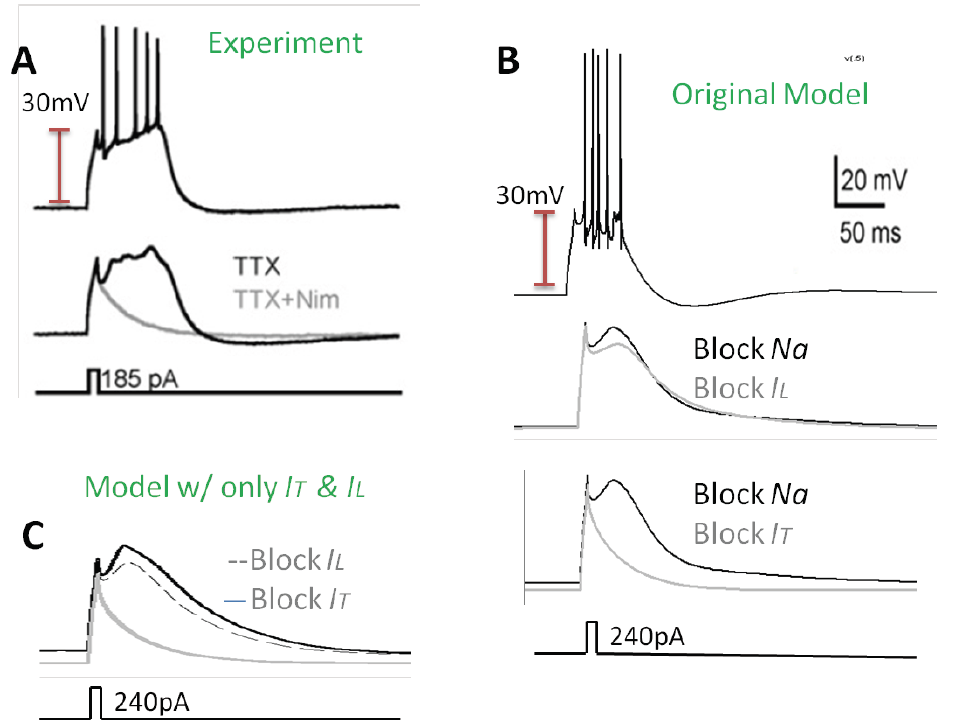
\includegraphics[scale=0.6]{chapters/chapter3/figures/fig1}} + \parbox{10mm}{\centering 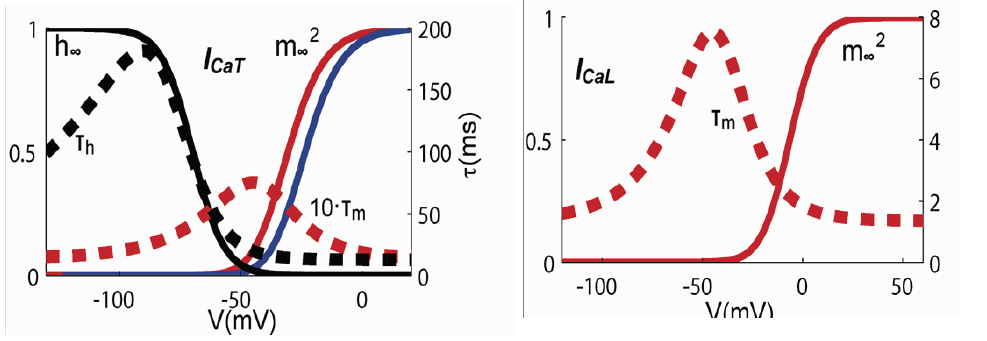
\includegraphics[scale=0.6]{chapters/chapter3/figures/fig2}} + \parbox{10mm}{\centering 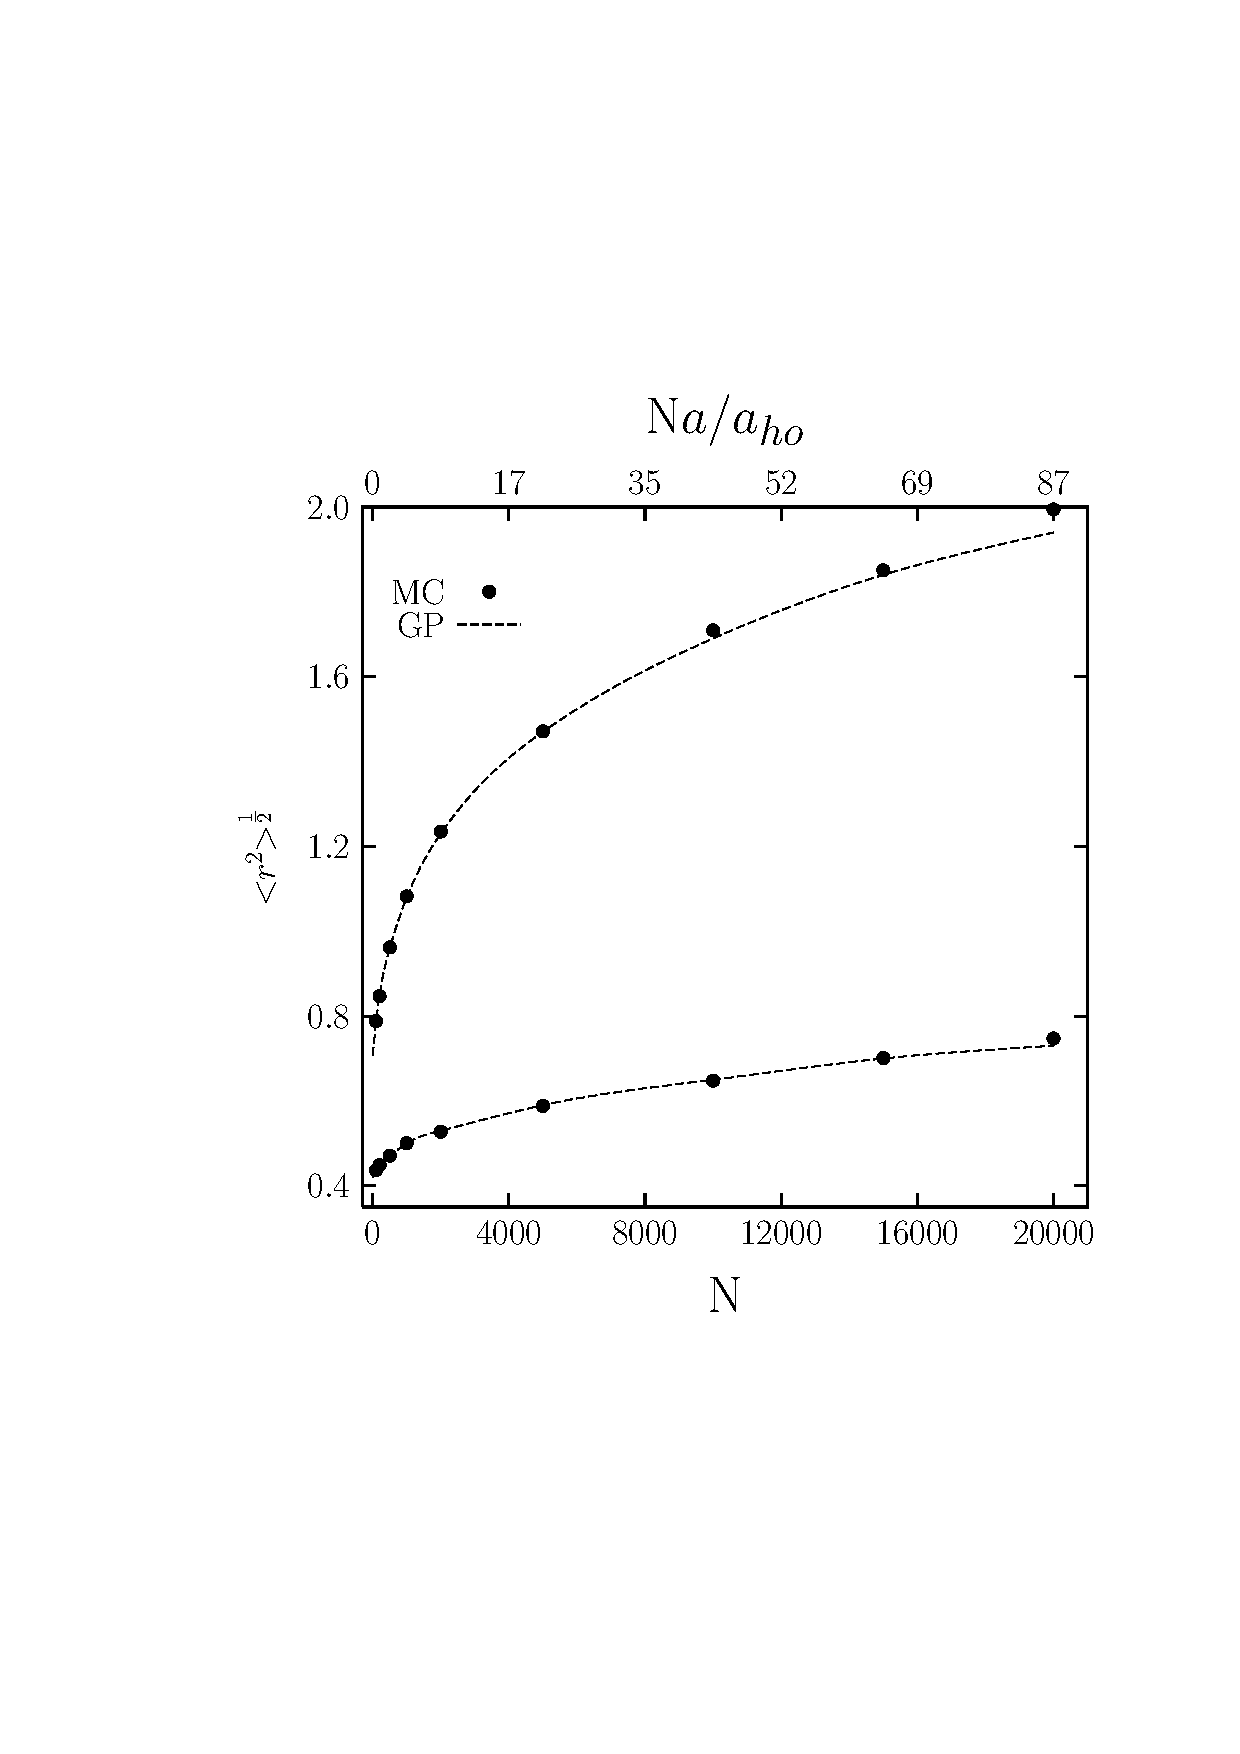
\includegraphics[scale=0.6]{chapters/chapter3/figures/fig3}} + \parbox{10mm}{\centering 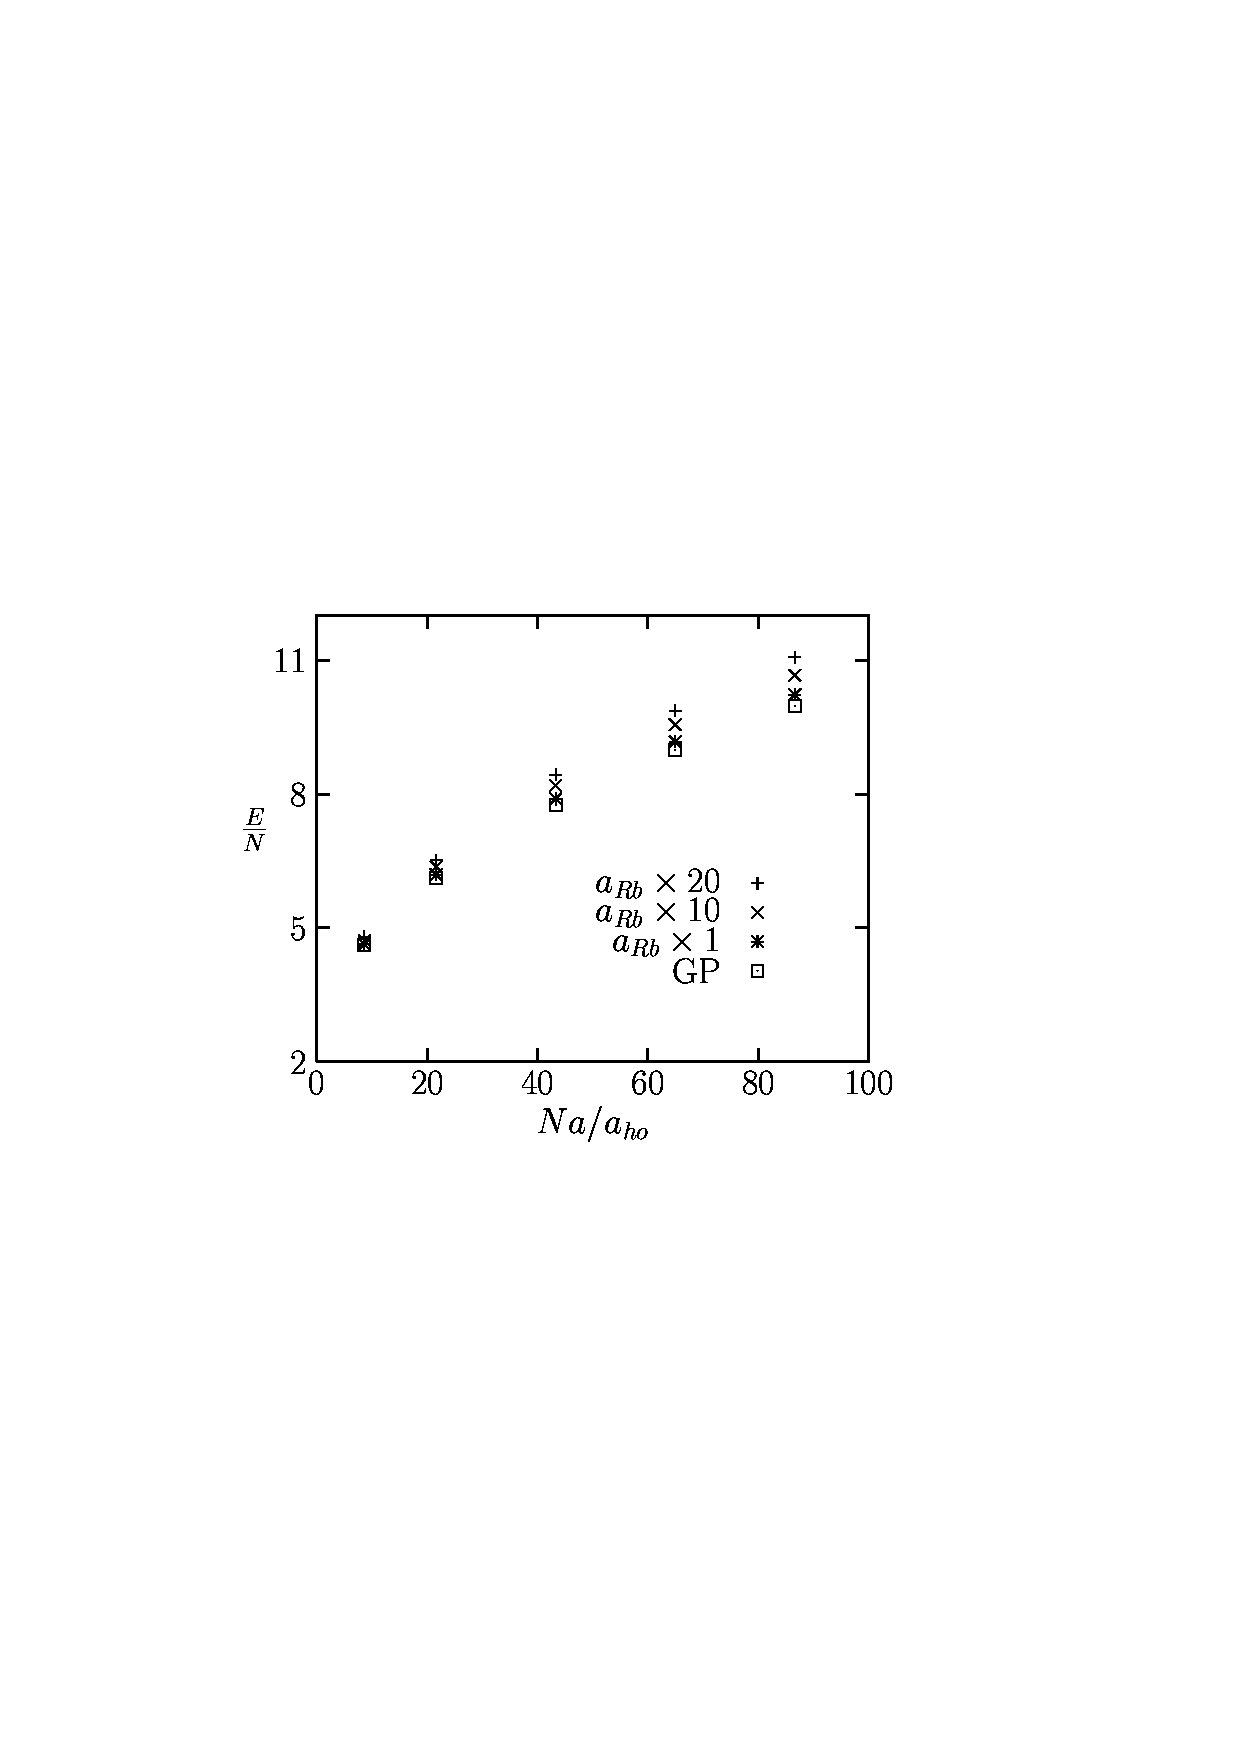
\includegraphics[scale=0.6]{chapters/chapter3/figures/fig4}} + \parbox{10mm}{\centering \includegraphics[scale=0.6]{chapters/chapter3/figures/dot}}  + \parbox{10mm}{\centering 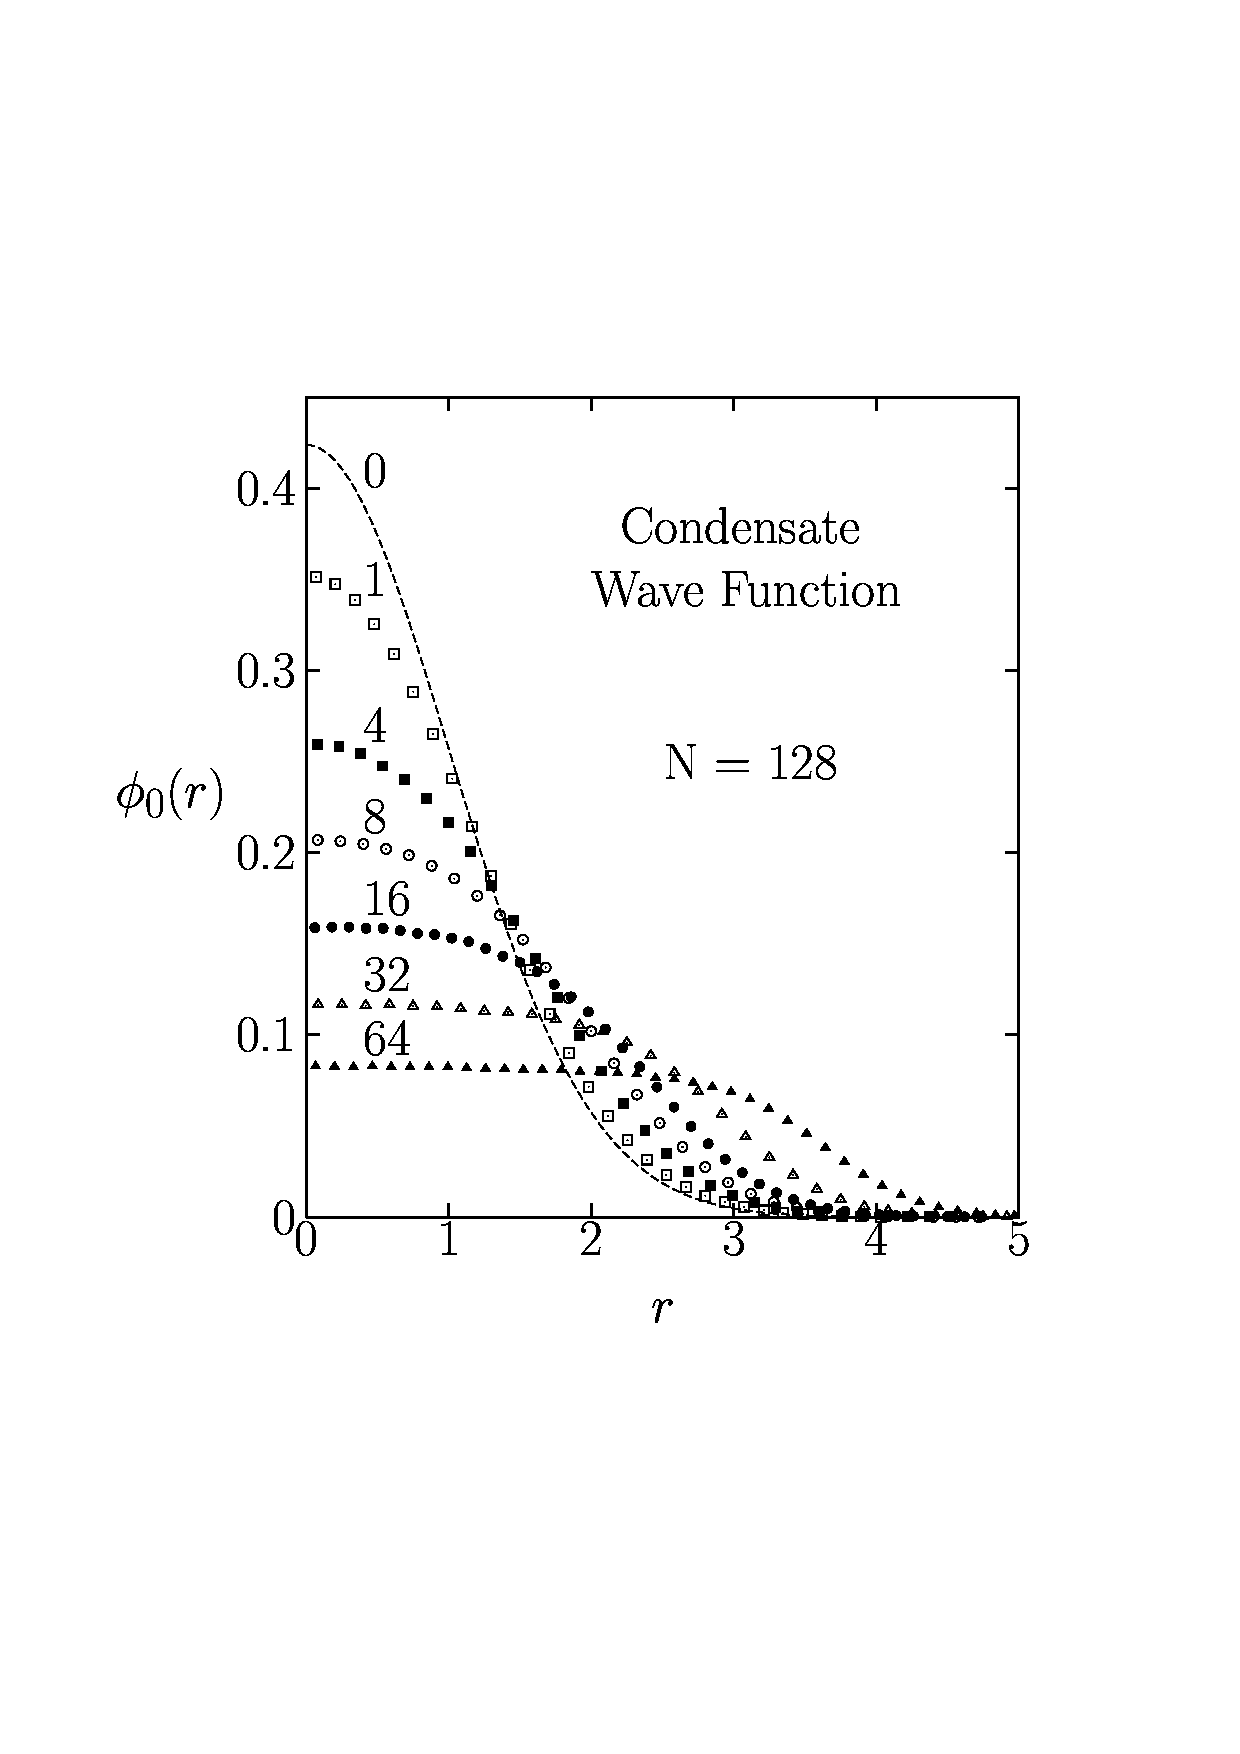
\includegraphics[scale=0.6]{chapters/chapter3/figures/fig5}} + \parbox{10mm}{\centering 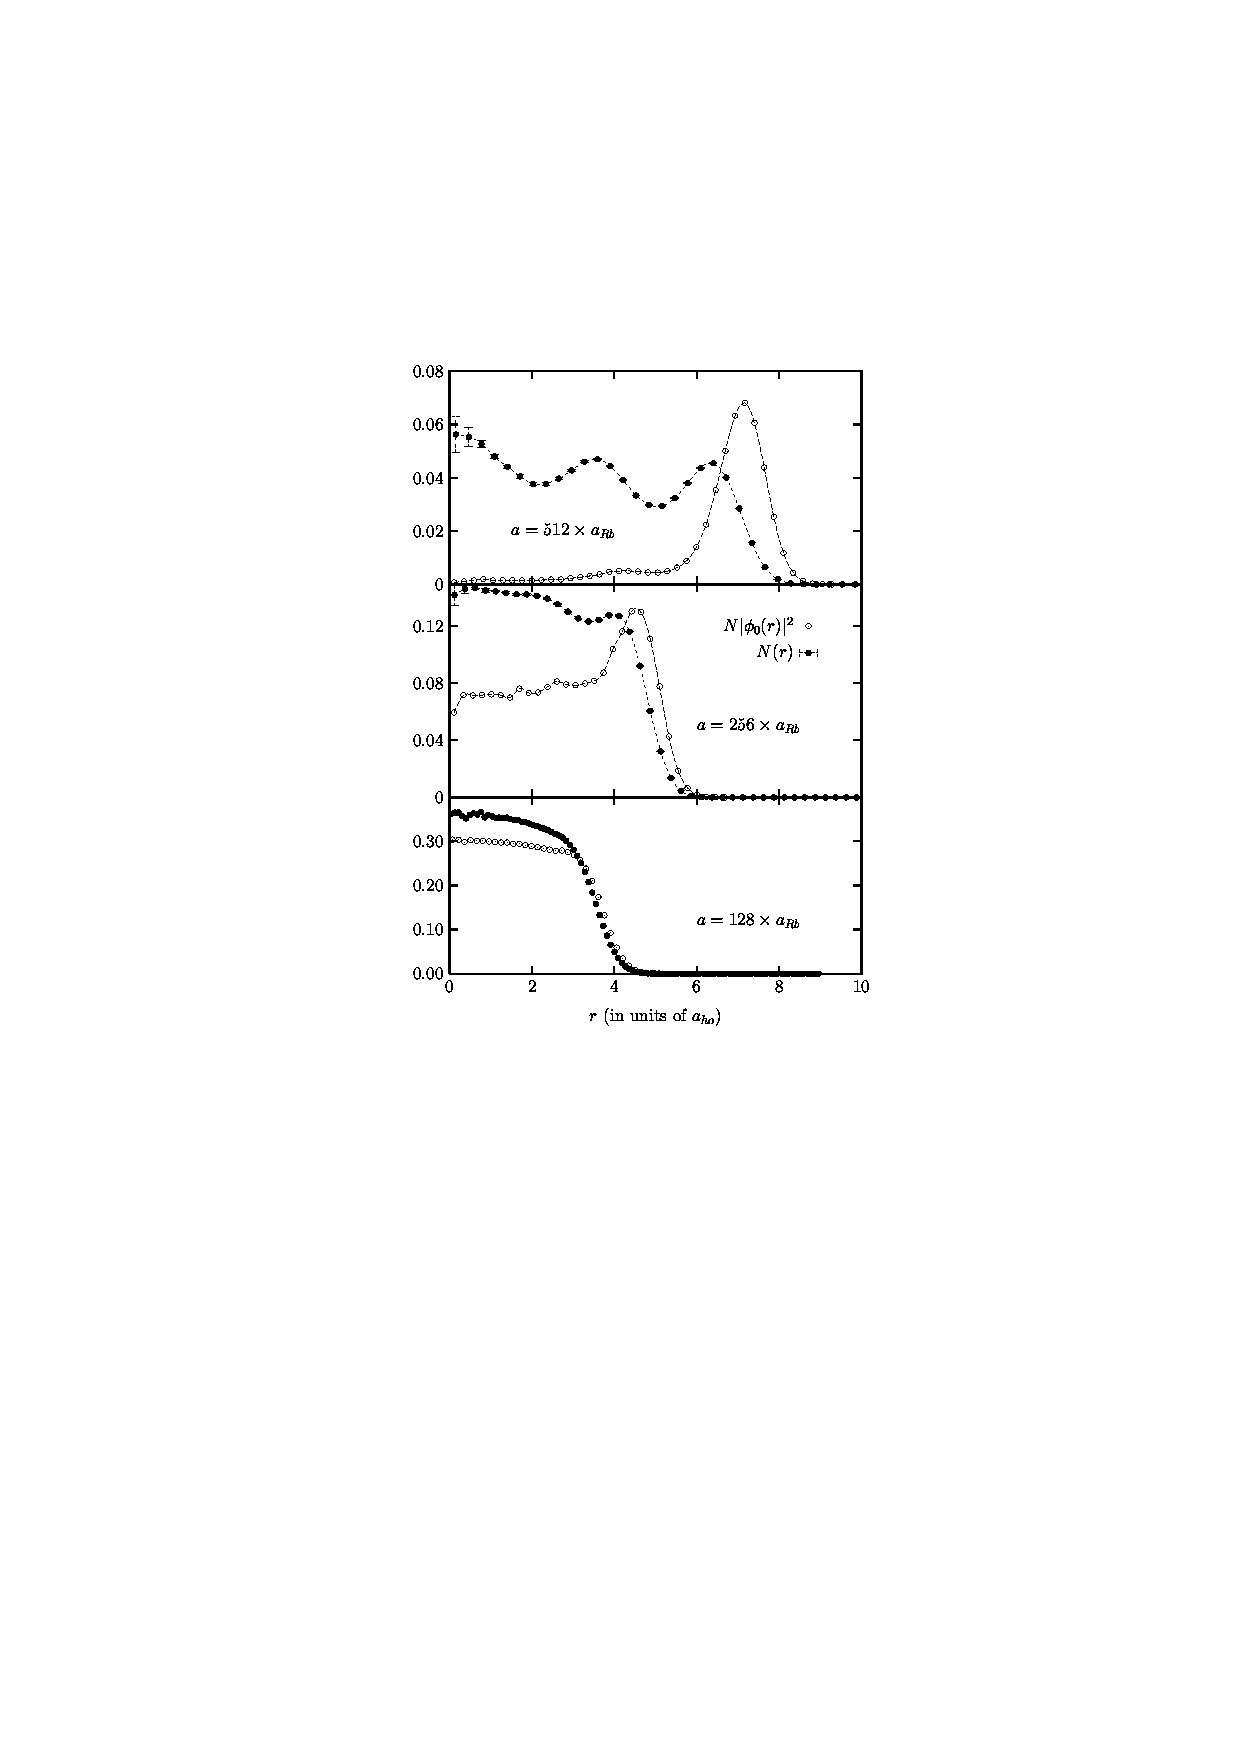
\includegraphics[scale=0.6]{chapters/chapter3/figures/fig6}} + \parbox{10mm}{\centering \includegraphics[scale=0.6]{chapters/chapter3/figures/dot}}  +  \parbox{10mm}{\centering 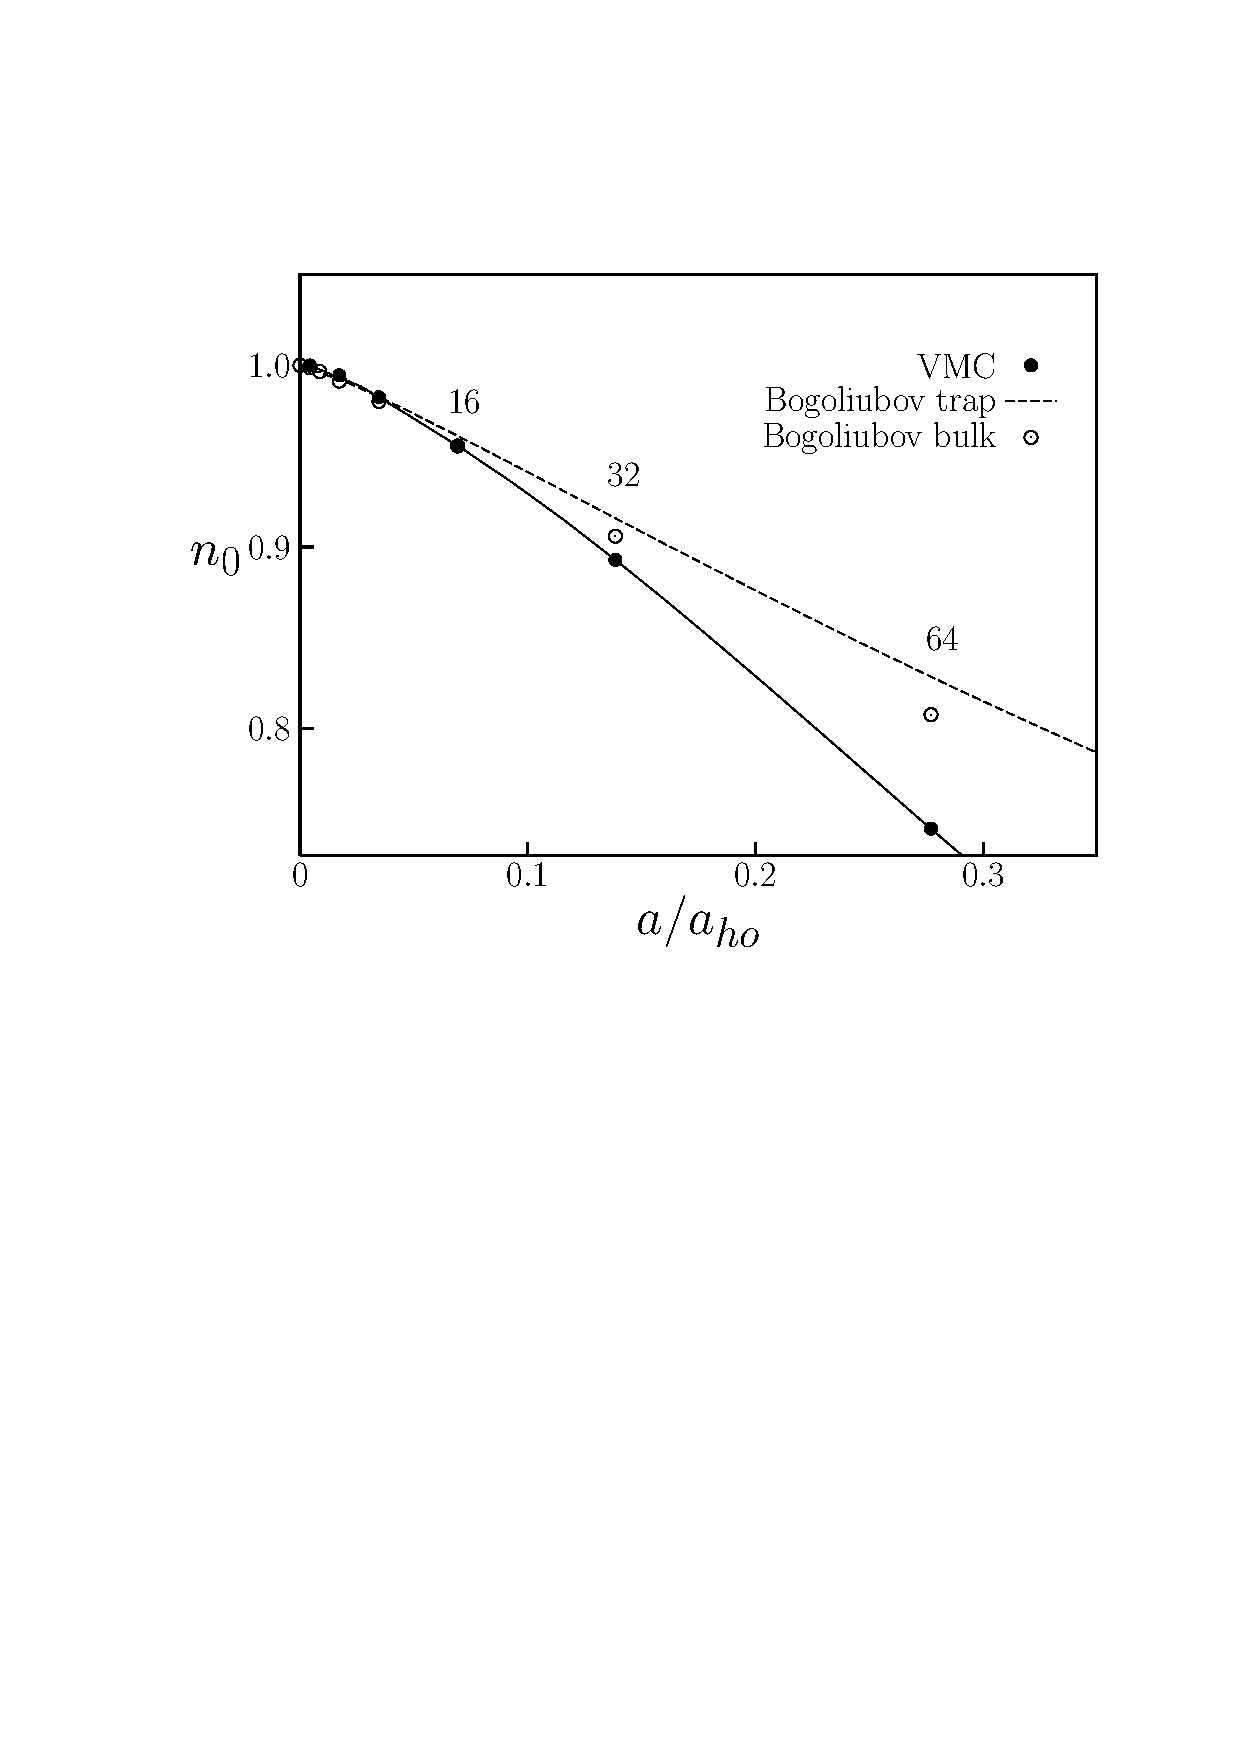
\includegraphics[scale=0.6]{chapters/chapter3/figures/fig7}} + \parbox{10mm}{\centering \includegraphics[scale=0.6]{chapters/chapter3/figures/dot}}\\
\notag
&+ \parbox{10mm}{\centering 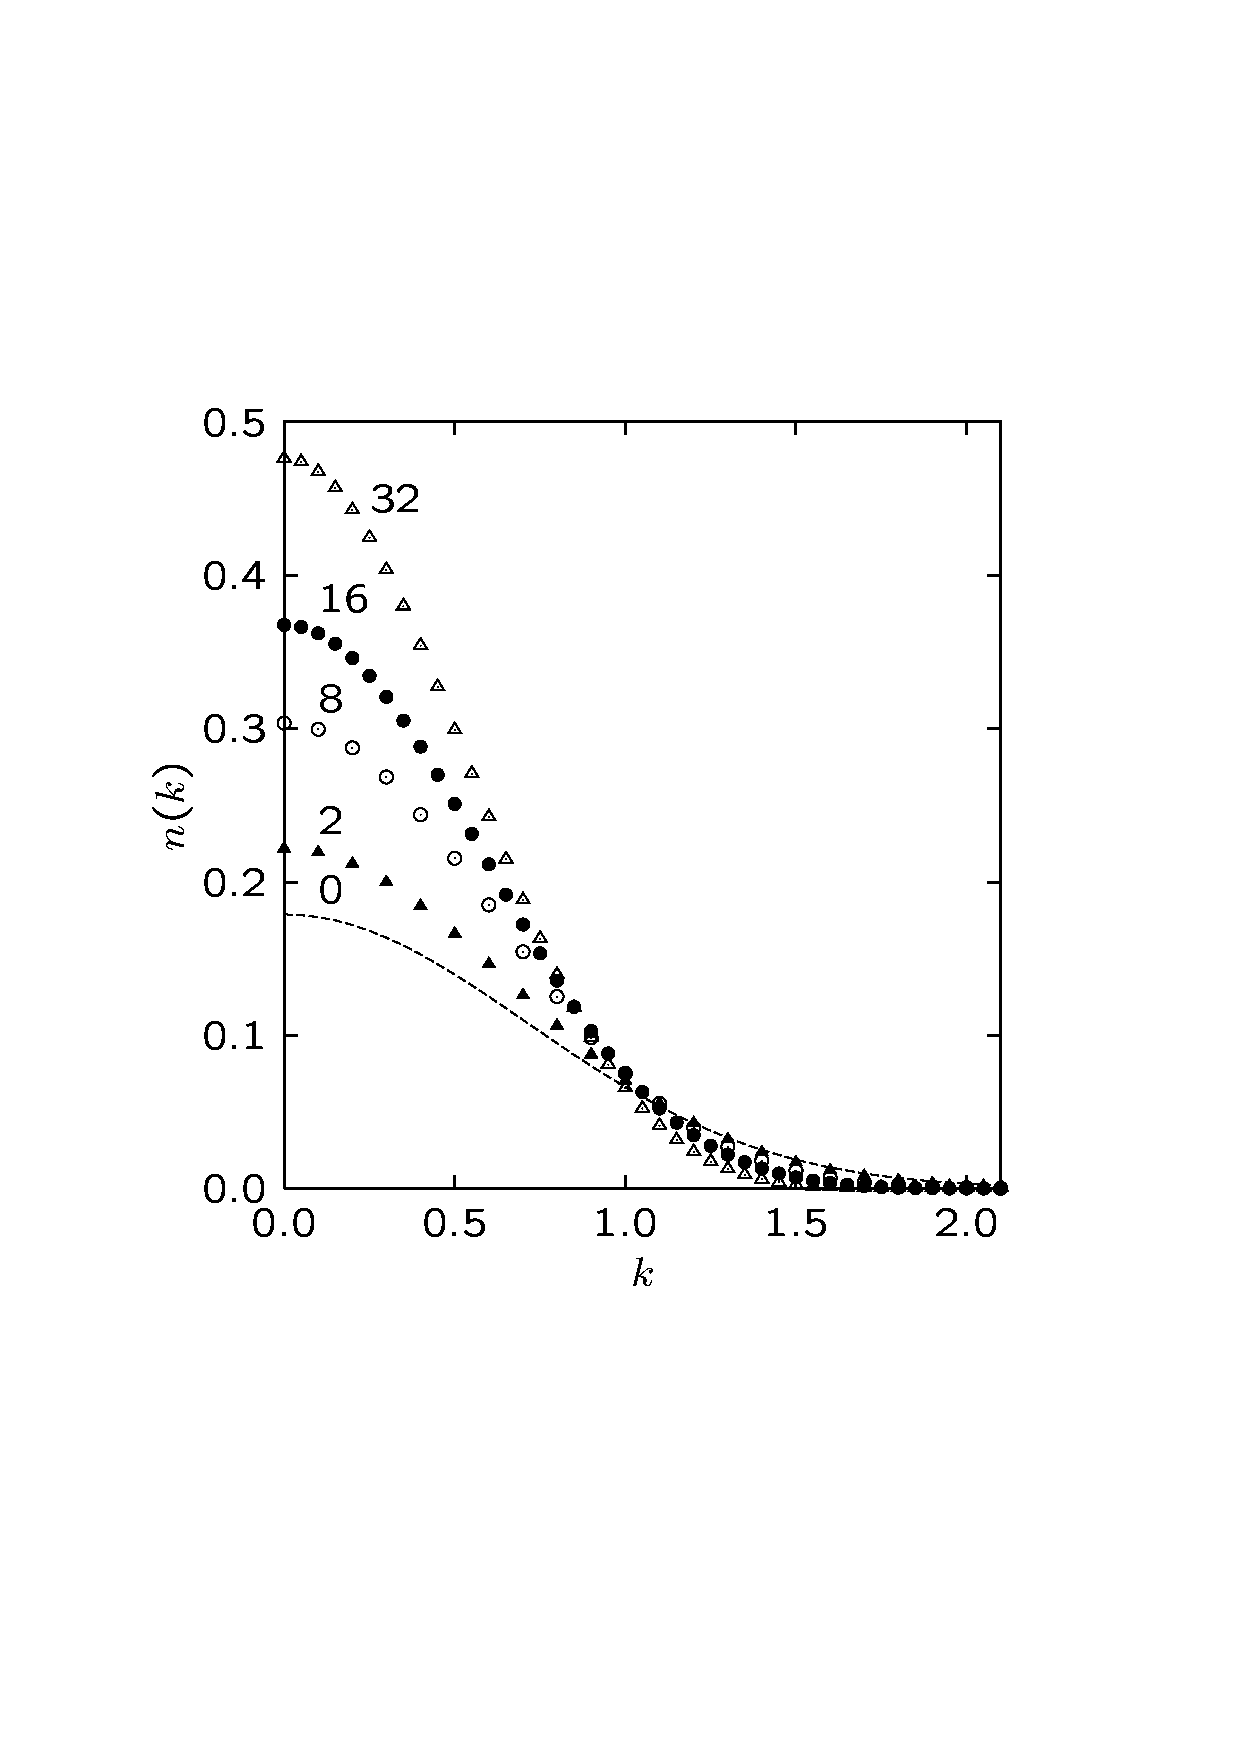
\includegraphics[scale=0.6]{chapters/chapter3/figures/fig9}} + \parbox{10mm}{\centering 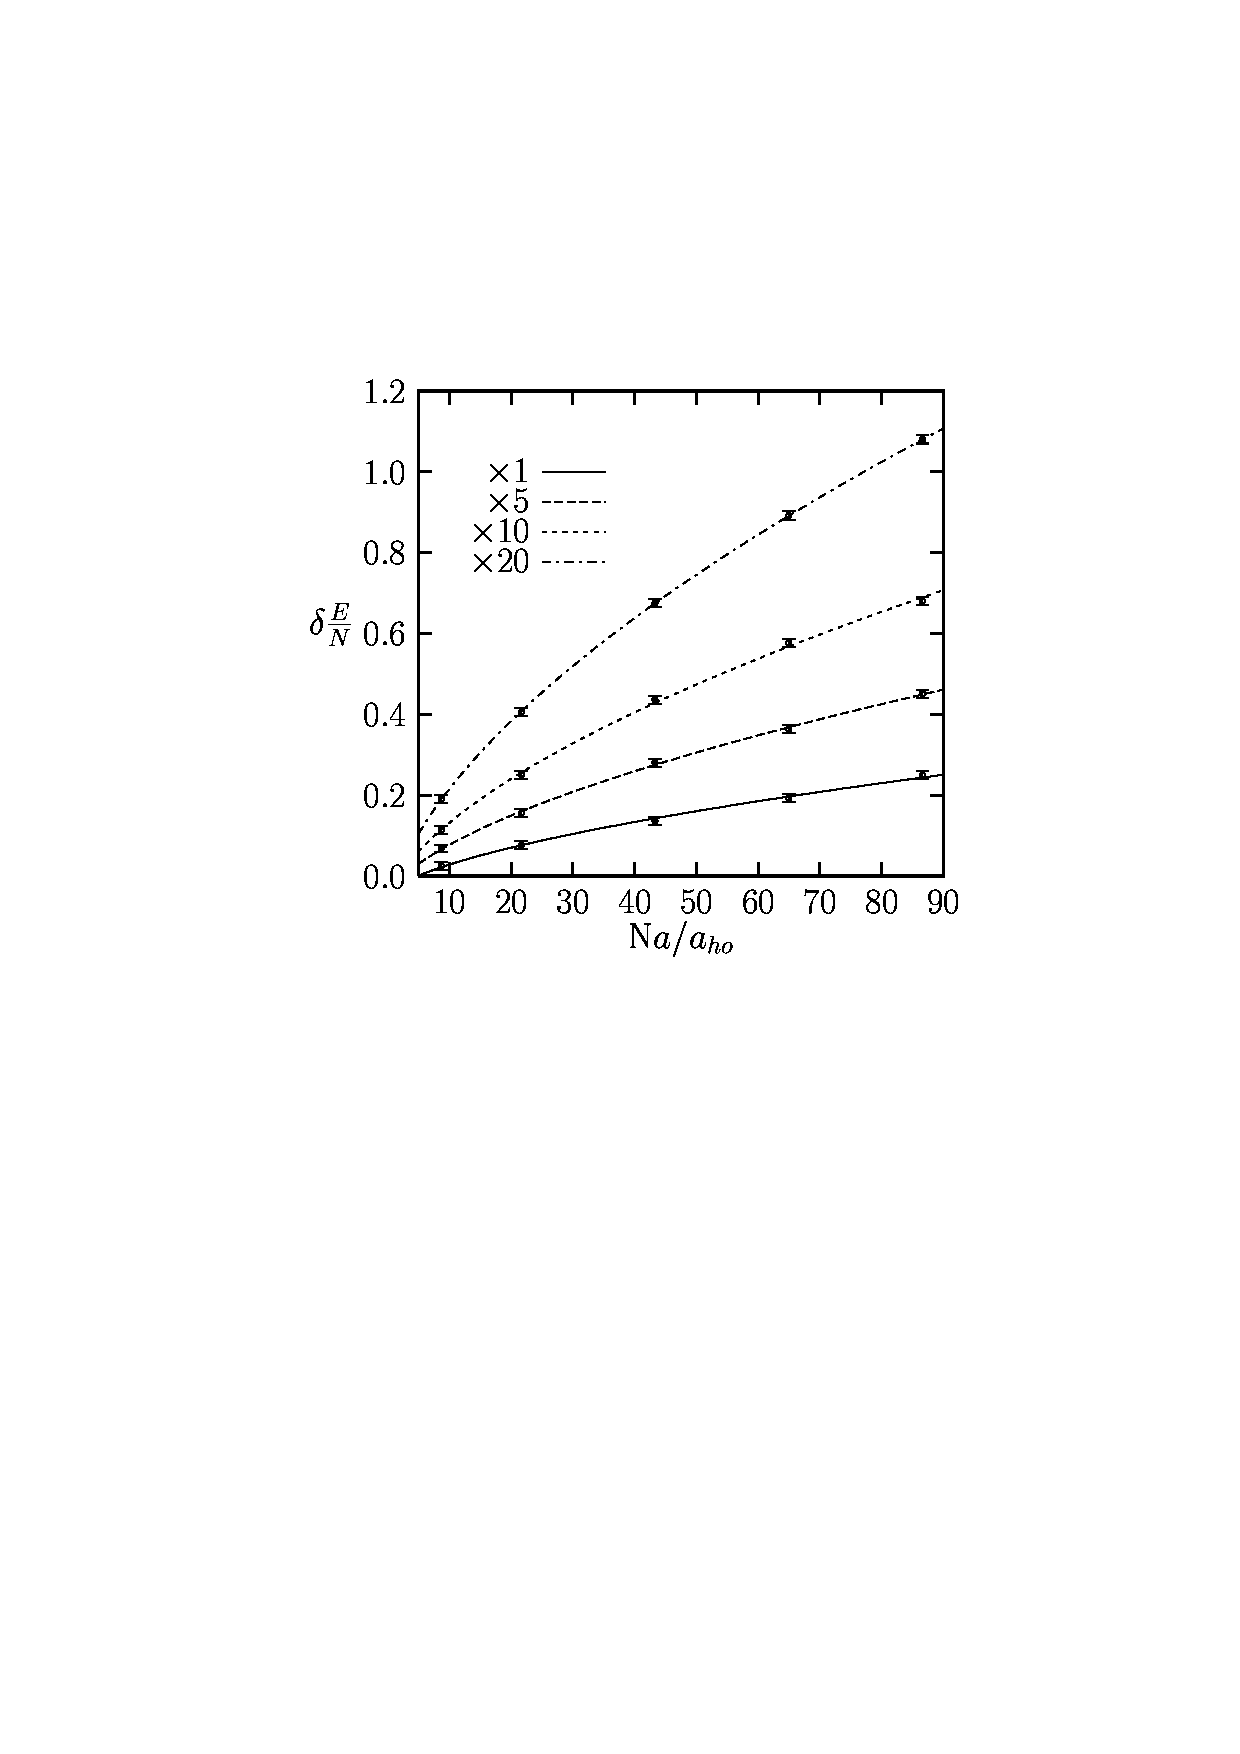
\includegraphics[scale=0.6]{chapters/chapter3/figures/fig10}} + \parbox{10mm}{\centering \includegraphics[scale=0.6]{chapters/chapter3/figures/dot}} + \parbox{10mm}{\centering \includegraphics[scale=0.6]{chapters/chapter3/figures/fig11}} + \parbox{10mm}{\centering \includegraphics[scale=0.6]{chapters/chapter3/figures/dot}} + \parbox{10mm}{\centering \includegraphics[scale=0.6]{chapters/chapter3/figures/fig13}} + \parbox{10mm}{\centering \includegraphics[scale=0.6]{chapters/chapter3/figures/fig14}} + \parbox{10mm}{\centering \includegraphics[scale=0.6]{chapters/chapter3/figures/dot}} + \parbox{10mm}{\centering \includegraphics[scale=0.6]{chapters/chapter3/figures/fig15}} + 
\parbox{10mm}{\centering \includegraphics[scale=0.6]{chapters/chapter3/figures/dot}}   \\
\notag
&+ \parbox{10mm}{\centering \includegraphics[scale=0.6]{chapters/chapter3/figures/fig16}} + \parbox{10mm}{\centering \includegraphics[scale=0.6]{chapters/chapter3/figures/fig17}} + \parbox{10mm}{\centering \includegraphics[scale=0.6]{chapters/chapter3/figures/dot}} + \parbox{10mm}{\centering \includegraphics[scale=0.6]{chapters/chapter3/figures/fig18}} + \parbox{10mm}{\centering \includegraphics[scale=0.6]{chapters/chapter3/figures/dot}} +  \parbox{10mm}{\centering \includegraphics[scale=0.6]{chapters/chapter3/figures/fig19}} + \parbox{10mm}{\centering \includegraphics[scale=0.6]{chapters/chapter3/figures/fig20}} + \parbox{10mm}{\centering \includegraphics[scale=0.6]{chapters/chapter3/figures/dot}} + \parbox{10mm}{\centering \includegraphics[scale=0.6]{chapters/chapter3/figures/fig21}} + \parbox{10mm}{\centering \includegraphics[scale=0.6]{chapters/chapter3/figures/dot}} \\
\notag
&+ \parbox{10mm}{\centering \includegraphics[scale=0.6]{chapters/chapter3/figures/dot}} + \parbox{10mm}{\centering \includegraphics[scale=0.6]{chapters/chapter3/figures/dot}} + \parbox{10mm}{\centering \includegraphics[scale=0.6]{chapters/chapter3/figures/fig22}} + \parbox{10mm}{\centering \includegraphics[scale=0.6]{chapters/chapter3/figures/fig23}} + \parbox{10mm}{\centering \includegraphics[scale=0.6]{chapters/chapter3/figures/fig24}} + \parbox{10mm}{\centering \includegraphics[scale=0.6]{chapters/chapter3/figures/fig25}} + \parbox{10mm}{\centering \includegraphics[scale=0.6]{chapters/chapter3/figures/fig26}} + \parbox{10mm}{\centering \includegraphics[scale=0.6]{chapters/chapter3/figures/dot}} + \parbox{10mm}{\centering \includegraphics[scale=0.6]{chapters/chapter3/figures/fig27}} + \parbox{10mm}{\centering \includegraphics[scale=0.6]{chapters/chapter3/figures/dot}}.
\end{align}
The horizontal lines represents the single-electron basis functions with spin included so that that each orbital can only be occupied by one electron at most. The non-interacting ground state is represented by the shaddowed area with a bold horizontal line denoting the fermie level of the system. The black circles obviously represents electrons, and the white ones represents holes. We will in following denote $n$-particle $n$-hole excitations by the shorthand notation $npnh$-excitations. The $1p1h$-excitations are unique in the sense that given a $1p1h$-excited determinant, we can only achieve this state by one distinct excitation. In the the $2p2h$ case, each excited state can be reached by two different excitations as indicated by the excitation lines. In the general case, one can a produce each $npnh$-excited state by $n!$ different ways of excitations. Physically, however, this is irrelevant since the only important information lies in the occupied single-electron states. Each diagram therefore represents $\textit{one}$ (excited) slater determinant with corresponding expansion coefficient included.  

Given the exact wave function $\ket{\Psi}$ and the complete set of slater determinants, the linear combination in Eq. (\ref{exp: Exact wave function}) is uniquely determined. However, the exact many-body wave function is $\textit{not}$ known, simply because this is the main objective in our calculation. In addition, as stated in chapter \ref{ch: Quantum Mechanics of Many-Body Systems}, the many-body problem can in most cases not be solved exactly. This imply that the infinite sum in Eq. (\ref{exp: Exact wave function}) cannot (necessarily) be determined exactly. At first sight, this does not look promising at all. The fact is, however, that Eq. (\ref{exp: Exact wave function}) serves as a fundamental starting point for several powerful and accurate $\textit{ab initio}$ methods such as configuration interaction (CI) and coupled-cluster (CC). The basic idea is that the exact wave function is approximated with a (necessarily) truncated determinantal expansion, and that the coefficients are determined by the Schr�dinger equation. Information of the electron-electron correlations hence lie in the expansion coefficients. Given the exact wave function one may always in principle tune these cofficients to yield the exact state. However, when the exact wave function is the objective, physical considerations must be build into these coefficients right from the beginning. Different approximations schemes serve as the origin for different many-body methods. Before we turn this point, basic notation are presented. 

%-----------------------
\subsection{Notation}
\label{subsec: Notation}
%-----------------------
We will in the following use the particle-hole formalism presented in section \ref{subsec: Particle-hole formalism}. The reference state is defined as 
\begin{align}
\ket{r} = \ket{\Phi},
\end{align}
where $\ket{\Phi_0}$ is the ground state of the non-interacting electronic system,
\begin{align}
\ket{\Phi_0} = \cre{\alpha_1}\cre{\alpha_2}..\cre{\alpha_N}\ket{0}.
\end{align}
The standard state-subscript from the particle-hole formalism is used; $i$,$j$,$k$,.. denot hole states and $a$,$b$,$c$,.. denote particle states. Hole states are single-electron orbitals that are occupied in the reference state, while particle states are all states beyond the fermi state. These subspaces is called occupied space and virtual space, respectively. States that are in either of the subspaces are denoted $p$,$q$,$r$,... We will not use the standard quasi-particle creation and annihilation operators $\crequasi{\alpha}$ and $\anquasi{\alpha}$ explicitly, but in an implicit way using vacuum creation and annihilation operators with quantum numbers $i,j,..,a,b,..,p,q,..$ indicating in which subspace they act. 
\begin{align}
\cre{i} &= \anquasi{\alpha} \hspace{0.5cm} \alpha\leq\alpha_F\\
\cre{a} &= \crequasi{\alpha} \hspace{0.5cm} \alpha>\alpha_F\\
\an{i} &= \crequasi{\alpha} \hspace{0.5cm} \alpha\leq\alpha_F\\
\an{a} &= \anquasi{\alpha} \hspace{0.5cm} \alpha>\alpha_F
\end{align}
We may now construct particle-, hole- and particle-hole (excited determinants) states by acting with strings of creation and annihilation operators on the reference state,
\begin{align}
\notag
\cre{a}\cre{b}\cre{c}..\ket{\Phi_0} &=  \parbox{10mm}{\centering \includegraphics[scale=0.2]{chapters/chapter3/figures/particleState}}& \hspace{1cm} \an{i}\an{j}\an{k}..\ket{\Phi_0}  &= \parbox{10mm}{\centering \includegraphics[scale=0.2]{chapters/chapter3/figures/holeState}}& \hspace{1cm} \cre{a}\cre{b}\cre{c}.. ..\an{k}\an{j}\an{i}\ket{\Phi_0} &= \parbox{10mm}{\centering \includegraphics[scale=0.2]{chapters/chapter3/figures/holeParticleState}}\\
\notag
&\equiv \ket{\Phi^{abc..}}& &\equiv \ket{\Phi_{ijk..}}& &\equiv \ket{\Phi_{ijk..}^{abc..}}
\end{align}
As shown above, particle-states will be denoted with virtual orbitals on the top right position of the state, hole-states with ocuupied orbitals in the lower right position, and particle-hole states with both virtual states and occupied states at their respective positions. The number of occupied and virtual orbitals yield the number of electrons in the system. For example, 
\begin{align}
\ket{\Phi_{n_o}^{n_v}},
\end{align}
represents a $(N+n_v-n_o)$-particle state, where $N$ is the number of particles in the reference state. When $n_v = n_o \neq 0$, the state represents an excitation of the reference state. 

%--------------------------------------------------------------------------------------------------------------------------------------------------------------
\section{Fundamental concepts}
\label{sec: fundamental concepts}
%--------------------------------------------------------------------------------------------------------------------------------------------------------------
We are seeking the solution of the Schr�dinger equation 
\begin{align}
\label{exp: Exact electronic Schr�dinger equation}
\OP{H}\ket{\Psi} = E\ket{\Psi},
\end{align}
for a system of $N$ interacting electrons in an external potential $u$. The hamiltonian written in second quantization (see section \ref{sec: Second Quantization}) reads 
\begin{align}
\label{exp: Electronic hamiltonian on second quantized form}
\OP{H} = \sum_{pq} \for{p}{h}{q} \cre{p}\an{q} + \frac{1}{4} \sum_{pqrs}\for{pq}{v}{rs}\cre{p}\cre{q}\an{s}\an{r},
\end{align}
where the two-body interaction elements are antisymmetrized. The one-body hamiltonian
\begin{align}
\label{exp: One-body hamiltonian}
\OP{h} = \OP{t} + \OP{u},
\end{align}
where $\OP{t}$ is the kinetic energy and $\OP{u}$ is the external one-body potential. The two-body interaction,
$\OP{v}$, is the well-known Coulomb interaction.

The many-electron problem can in general not be solved exactly, which imply that the energy eigenfunctions cannot be
written down in an analytically closed form. However, as pointed out in the introduction to this chapter, given an 
arbitrary orthonormal and complete set of single-electron functions, the exact energy
eigenfunctions can be expanded in an infinite series (\ref{exp: Exact wave function}) of slater determinants constructed from these. We choose the
single-electron basis to be the set of energy eigenfunctions determined by the single-particle Schr�dinger equation
\begin{align}
\OP{h}\ket{\phi_\alpha} = \epsilon_\alpha \ket{\phi_\alpha},
\end{align}
with $\OP{h}$ defined in Eq. (\ref{exp: One-body hamiltonian}). Hence, according to Eq. (\ref{exp: Exact wave function}) 
and the schematic drawing in Eq. (\ref{exp: Exact wave function, schematic drawing}), the exact wave function can be 
written as a linear combination of all possible exciations (energy eigenstates) of the non-interacting system. Applying the
notation presented in the previous chapter, Eq. (\ref{exp: Exact wave function}) reads
\begin{align}
\label{exp: Exact wave function, new notation}
\ket{\Psi} = C_0\ket{\Phi} + \sum_{ia}C_i^a\ket{\Phi_i^a} + \sum_{ijab}C_{ij}^{ab}\ket{\Phi_{ij}^{ab}} + ... + 
\sum_{ijk..abc..}C_{ijk..}^{abc..}\ket{\Phi_{ijk..}^{abc..}},
\end{align}
where the infinite series of determinantal functions naturally terminates when all particles are excited. The first sum
represents $1p1h$-excitations, the second $2p2h$-exciations, and so forth up to $NpNh$-excitations. Even though the 
expansion is finite in order of particle-hole excitations, it is still infinite in the virtual orbitals $a,b,c..$. If we 
were able to go to infinity in the virtual orbitals, the exact wave function is given by Eq. (\ref{exp: Exact wave function, new notation}).
However, Eq. (\ref{exp: Exact wave function, new notation}) is not complete in the sense that it does not give any 
information about what contributes to the individual expansion coefficients. It simply tell us that given the exact
wave function we can in principle always tune each coefficient iteself without explicitly calculating its different contributions, 
so that the linear expansion of determinantal functions yield the exact state. The wave function is however $\textit{not}$ known, which imply that the coefficients are the unknowns to be determined by the Schr�dinger equation. Before this can be done, we must specify what contributes to each expansion coefficients $C_{ij..}^{ab..}$. For a given excited slater determinant $\ket{\Phi_{ij..}^{ab..}}$, the corresponding expansion coefficients $C_{ij..}^{ab..}$ gets contributions from $\textit{excitation amplitudes}$ with all possible electron-electron correlation. As an example, consider the $3p3h$-excited determinant $\ket{\Phi_{ijk}^{abc}}$. The corresponding expansion coefficient $C_{ijk}^{abc}$ gets contributions from excitation amplitudes with all possible electron-electron ,
\begin{align}
C_{ijk}^{abc} = t_i^at_j^bt_k^c + t_{ij}^{ab}t_k^c + t_i^at_{jk}^{bc} + t_j^bt_{ik}^{ac} + t_{ijk}^{abc}
\end{align}
The coupling can shematically be shown by,
\begin{align}
C_{ijk}^{abc}\ket{\Phi_{ijk}^{abc}} &= \pr{t_i^at_j^bt_k^c + t_{ij}^{ab}t_k^c + t_i^at_{jk}^{bc} + t_j^bt_{ik}^{ac} + t_{ijk}^{abc}}\ket{\Phi_{ijk}^{abc}} \\ 
\label{exp: Expansion coefficients coupling}
&=
\parbox{10mm}{\centering \includegraphics[scale=0.2]{chapters/chapter3/figures/particleCoupling}} + 
\parbox{10mm}{\centering \includegraphics[scale=0.2]{chapters/chapter3/figures/particleCoupling2}} + 
\parbox{10mm}{\centering \includegraphics[scale=0.2]{chapters/chapter3/figures/particleCoupling3}} + 
\parbox{10mm}{\centering \includegraphics[scale=0.2]{chapters/chapter3/figures/particleCoupling4}} +
\parbox{10mm}{\centering \includegraphics[scale=0.2]{chapters/chapter3/figures/particleCoupling5}}.
\end{align}
Each the figures in Eq. (\ref{exp: Expansion coefficients coupling}) denote the contribution to the total expansion coefficient $C_{ijk}^{abc}$ from one of the possible correlations of electrons within specific orbitals. The first figure in Eq. (\ref{exp: Expansion coefficients coupling}) represents the excited slater determinant with three $1p1h$-excitation amplitudes that do not couple any of the electrons. This is a crucial contribution when we consider a system consisting of two subsystems that do not interact with each other. In addition, a weakly interacting system may get important contribution to the $3p3h$ from $3$ independent $1p1h$-excitations. The second, third and forth term in Eq. (\ref{exp: Expansion coefficients coupling}) denote the excited determinant where the motions of two electrons within selected pair of orbitals are correlated. The fifth term represents the contribution the expansion coefficient where all electrons are coupled. This example illustrates that for a given $npnh$-excited slater determinant, one may produce this state by correlating the motion of electrons within specific orbitals in all possible ways. The corresponding expansion coefficient hence gets contributions from excitation amplitudes with all possible electron-electron coupling. 

We now define the single-orbital excitation operator (cluster operator)
\begin{align}
\OP{t}_i = \sum_a t_i^a \cre{a}\an{i},
\end{align}
which acting on the reference state yields,
\begin{align}
\OP{t}_i\ket{\Phi} = \sum_a t_i^a \ket{\Phi_i^a}. 
\end{align}
Similarly, we define the two-orbital excitation operator, which couple the pair of excited electrons, as
\begin{align}
 \OP{t}_{ij}^{ab} = \frac{1}{2}\sum_{ab}t_{ij}^{ab}\cre{a}\cre{b}\an{j}\an{i},
\end{align}
which acting on the reference state yields 
\begin{align}
\OP{t}_{ij}^{ab}\ket{\Phi} = \frac{1}{2}\sum_{ab}t_{ij}^{ab}\ket{\Phi_{ij}^{ab}},
\end{align}
where the motion of the excited pair of electrons are correlated. In general case, the $n$-orbital excitation operator is defined as
\begin{align}
\OP{t}_{ijk..}^{abc..} = \frac{1}{n!}\sum_{abc..}t_{ijk..}^{abc..}\cre{a}\cre{b}\cre{c}....\an{k}\an{j}\an{i}.
\end{align}
When acting on the reference state it produces all $npnh$-excitations (with holes in i,j,k,..) where the motions of all excited electrons are correlated with each other,
\begin{align}
\OP{t}_{ijk..}^{abc..}\ket{\Phi} = \frac{1}{n!}\sum_{abc..}t_{ijk..}^{abc..}\ket{\Phi_{ijk..}^{abc..}}. 
\end{align}
These excitation operators allow us to produce excited determinants with all possible electron-electron coupling. For example, 
\begin{align}
\pr{\OP{t}_i\OP{t}_j + \OP{t}_{ij}}\ket{\Phi} = \frac{1}{2}\sum_{ab}\pr{t_i^at_j^b + t_{ij}^{ab}}\ket{\Phi_{ij}^{ab}},
\end{align}
produces all $2p2h$-excited determinants with a hole-pair in $i$ and $j$. In addition, by summing over $i$ and $j$, we obtain all $2p2h$-states
\begin{align}
\frac{1}{4}\sum_{ijab}\pr{t_i^at_j^b + t_{ij}^{ab}}\ket{\Phi_{ij}^{ab}}.
\end{align}
It is therefore appropriate to define $\textit{total}$ excitation amplitudes,
\begin{align}
\OP{T}_1 &\equiv \sum_i \OP{t}_i = \sum_{ia}t_i^a\cre{a}\an{i}\\
\OP{T}_2 &\equiv \frac{1}{2}\sum_{ij}\OP{t}_{ij}^{ab} = \frac{1}{4}\sum_{ijab}t_{ij}^{ab}\cre{a}\cre{b}\an{j}\an{i}\\
\notag
&\vdots \hspace{1cm} \vdots \\
\OP{T}_n &\equiv \frac{1}{n!}\sum \OP{t}_{ijk..}^{abc..}\cre{a}\cre{b}\cre{c}....\an{k}\an{j}\an{i} =  \pr{\frac{1}{n!}}^2\sum_{ijk..abc..}t_{ijk..}^{abc..}\cre{a}\cre{b}\cre{c}....\an{k}\an{j}\an{i}.
\end{align}
The total excitation amplitudes can be used to obtain all-order excitations with all possible coupling between the electrons. For example, all $3p3h$-excitations is obtained by using combining $\OP{T}_1$, $\OP{T}_2$ and $\OP{T}_3$,
\begin{align}
\ket{3p3h} = \pr{\frac{1}{6}\OP{T}_1^3 + \OP{T}_1\OP{T}_2 + \OP{T}_3}\ket{\Phi_0}. 
\end{align}
In the general case, all $npnh$-excitations with all possible correlations are generated by combining $\OP{T}_1$, $\OP{T}_2$, ..., $\OP{T}_n$. 

We can now rewrite the exact wavefunction (\ref{exp: Exact wave function, new notation}) in terms of total excitation operators. It is at this point the difference between configuration interaction and coupled-cluster appears. The configuration interaction method builds up the wavefunction with only fully correlated electrons, i.e. no products of excitation excitation operators. The CI wavefunction reads
\begin{align}
\ket{\Psi}_{CI} = \pr{1 + \OP{T}_1 + \OP{T}_2 + \OP{T}_3 + ... + \OP{T}_N}\ket{\Phi_0}.
\end{align}
The coupled-cluster method, however, also include products of excitation operators, so that the CC wavefunction is given by
\begin{align}
\label{exp: Coupled-cluster wavefunction}
\ket{\Psi}_{CC} &= \Big(1 + \OP{T}_1 + \fpr{\frac{1}{2!}\OP{T}_1^2 + \OP{T}_2} + \fpr{\frac{1}{3!}\OP{T}_1^3 + \OP{T}_1\OP{T}_2 + \OP{T}_3}\\ &+ \fpr{\frac{1}{4!}\OP{T}_1^4 + \frac{1}{2!}\OP{T}_1^2\OP{T}_2 + \OP{T}_1\OP{T}_3 + \frac{1}{2!}\OP{T}_2^2 + \OP{T}_4} + ... + \fpr{... + \OP{T}_N}\Big)\ket{\Phi}.
\end{align}
Higher-order terms (like $\OP{T}_{N+1}$) do not appear since $N$ is the number of electrons in the system. Because all excitation operators commute, all terms in Eq. (\ref{exp: Coupled-cluster wavefunction}) match those from the power series expansion of an exponental function. Thus, the $\textit{exact}$ wavefunction can be written as
\begin{align}
\label{exp: Coupled-cluster wavefunction 2}
\ket{\Psi} = e^{\OP{T}}\ket{\Phi},
\end{align}
where 
\begin{align}
\label{exp: Excitation operators}
\OP{T} = \OP{T}_1 + \OP{T}_2 + ... + \OP{T}_N.
\end{align}
The wavefunction in Eq. (\ref{exp: Coupled-cluster wavefunction 2}) is usually called the $\textit{coupled-cluster wavefunction}$ or the $\textit{exponential ansatz}$. In practical calculations we are obviously forced to choose a model space $\mathcal{P} \subset \mathcal{H}_N$, which is equivalent to truncate the summations in the excitation amplitudes in a specific way. In addition, when the system consists of many particles, we are often forced to truncate the total excitation operator $\OP{T}$ in Eq. (\ref{exp: Excitation operatxcitation operators}). Both the way we choose our model space $\mathcal{P}$ and where we truncate the total excitation operator $\OP{T}$ have consequences for our calculations. At this point, we just emphasize that in practical calculations, the $\textit{exact}$ wavefunction 
\begin{align}
\ket{\Psi} \neq e^{\OP{T}}\ket{\Phi}.
\end{align}
We therefore define the $\textit{coupled-cluster wavefunction}$ as
\begin{align}
\ket{\Psi}_{CC} \equiv e^{\OP{T}}\ket{\Phi},
\end{align}
where 
\begin{align}
\OP{T} = \OP{T}_1 + \OP{T}_2 + ... + \OP{T}_i \hspace{1cm} i\leq N.
\end{align}
This is an $\textit{ansatz}$ to the exact wavefunction. Our hope is that most of the correlations in the system are baked into the coupled-cluster wavefunction so that
\begin{align}
\ket{\Psi} \approx \ket{\Psi}_{CC}.
\end{align}
How ``good'' our coupled-cluster ansatz is, are completely determined by our model space $\mathcal{P}$ and where the total excitation operator $\OP{T}$ is truncated. Truncation at specific excitation level leads to a hierarchy of basic coupled-custer schemes,
\begin{align}
\OP{T} &= \OP{T}_1 + \OP{T}_2 \rightarrow CCSD\\
\OP{T} &= \OP{T}_1 + \OP{T}_2 + \OP{T}_3 \rightarrow CCSDT\\
\OP{T} &= \OP{T}_1 + \OP{T}_2 + \OP{T}_3 + \OP{T}_4 \rightarrow CCSDTQ\\
\notag
\OP{T} &= \OP{T}_1 + \OP{T}_2 + \OP{T}_3 + \OP{T}_4 + ... + \OP{T}_N \rightarrow CCSDTQ..N
\end{align}
where $S$, $D$, $T$ and $Q$ denote single-, double-, triple- and quadruple-excitations, respectively. In the next section, the formal theory of coupled-cluster is presented. 

%------------------------------------------------------------------------------------------------------------------------------------------------------
\section{The formal coupled-cluster theory}
\label{sec: the formal coupled-cluster theory}
%------------------------------------------------------------------------------------------------------------------------------------------------------
The coupled-cluster wavefunction given in Eq. (\ref{exp: Coupled-cluster wavefunction 2}) is the starting point for all CC calculations. First we approximate the exact wavefunction with the CC wavfunction,
\begin{align}
\ket{\Psi} \approx \ket{\Psi}_{CC} = e^{\OP{T}}\ket{\Phi},
\end{align}
which hopefully, but not a priori, is a good approximation. We now substitute the coupled-cluster wavefunction into the Schr�dinger equation, yielding
\begin{align}
\label{exp: Coupled-cluster schr�dinger equation}
\OP{H}e^{\OP{T}}\ket{\Phi} = Ee^{\OP{T}}\ket{\Phi},
\end{align}
where $E$ is the energy eigenvalue. The unknowns are the excitation amplitudes ($t_i^a t_{ij}^{ab}..t_{ijk..}^{abc..}$) and the energy $E$, which are determined by Eq. (\ref{exp: Coupled-cluster schr�dinger equation}). The basic CC equations are the so-called $\textit{energy equation}$ and the $\textit{amplitude equations}$, which constitute the basic CC machinery. The formal form of the equations is found be using a ``projective'' technique where Eq. (\ref{exp: Coupled-cluster schr�dinger equation}) is projected down on an eigenstate of the non-interacting system. The energy equation is found by multiplying the equation with the dual reference state from the left, yielding 
\begin{align}
\label{exp: Formal CC energy equation}
\for{\Phi}{\OP{H}e^{\OP{T}}}{\Phi} = E\for{\Phi}{e^{\OP{T}}}{\Phi} = E.
\end{align}
The last equality in Eq. (\ref{exp: Formal CC energy equation}) follows from the fact that $\indre{\Phi}{\Psi}_{CC} = 1$, by construction. Expressions for the excitation amplitudes is obtained in a similar fashion by left-projecting the Schr�dinger equation down on the excited determinants produced when $\OP{T}$ acts on the reference state,
\begin{align}
\label{exp: Formal CC amplitude equation}
\for{\Phi_{ijk..}^{abc..}}{\OP{H}e^{\OP{T}}}{\Phi} = E\for{\Phi_{ijk..}^{abc..}}{e^{\OP{T}}}{\Phi} = Et_{ijk..}^{abc..}.
\end{align}
Due to the presence of $e^{\OP{T}}$, each amplitude equation for a specific $t_{ijk..}^{abc..}$ couple the amplitude to other excitation amplitudes. The CC equation must therefore be solved iteratively. Again we emphasize that the equations are formally $\textit{exact}$. When $\OP{T}$ is not truncated, the exact wavefunction within our model space $\mathcal{P}$ may be found. 

Eq. (\ref{exp: Formal CC energy equation}) and Eq. (\ref{exp: Formal CC amplitude equation} serves only as a way to get formal insight into the CC method. In practical computer implementation, however, they are not useful \cite{Schaefer}. The first step to obtain programable equations is to multiply Eq. (\ref{exp: Coupled-cluster schr�dinger equation}) with $e^{-\OP{T}}$ from the left, and the use the ``projective'' technique. The modified energy and amplitude equations reads
\begin{align}
\label{exp: Conventional CC energy equation}
\for{\Phi}{e^{-\OP{T}}\OP{H}e^{\OP{T}}}{\Phi} &= E\\
\label{exp: Conventional CC amplitude equation}
\for{\Phi_{ijk..}^{abc..}}{e^{-\OP{T}}\OP{H}e^{\OP{T}}}{\Phi} &= 0,
\end{align}
where the projection onto the excited determinant $\ket{\Phi_{ijk..}^{abc..}}$ yield the expression for the amplitude $t_{ijk..}^{abc..}$ (coupled to other amplitudes). Eq. (\ref{exp: Conventional CC energy equation}) and Eq. (\ref{exp: Conventional CC amplitude equation}) define the conventional CC method. Furtheremore, these equations are equivalent to the formal equations in Eq. (\ref{exp: Formal CC energy equation}) and Eq. (\ref{exp: Formal CC amplitude equation}) \cite{Schaefer}, but have two advantages important for practical calculation. First, the amplitude equations are decoupled from the energy equation. Second, the similarity transformed hamiltonian $e^{-\OP{T}}\OP{H}e^{\OP{T}}$ can be re-written by the so-called Campbell-Baker-Hausdorff (CBH) expansion as a sum of nested commutators which, as we will observe shortly, truncates naturally. This yields a considerable simplifications of the equations. 
 
%%%%%%%%%%%%%%%%%%%%%%%%%%%%%%%%%%%%%%%%%%%
\section{The coupled-cluster equations}
\label{sec: the coupled-cluster equations}
%%%%%%%%%%%%%%%%%%%%%%%%%%%%%%%%%%%%%%%%%%%
We will in this section derive the coupled-cluster singles and doubles (CCSD) equations with both an algebraic and diagramatic approach. The methods are completely general and may be extended to derive higher-order equations such as CCSDT, CCSDTQ and so forth. In CCSD we define the total excitation operator as 
\begin{align}
\OP{T} \equiv \OP{T}_1 + \OP{T}_2,
\end{align}
where 
\begin{align}
\label{exp: T1 excitation operator}
\OP{T}_1 &= \sum_{ia}t_i^a \cre{a}\an{i}\\
\label{exp: T2 excitation operator}
\OP{T}_2 &= \frac{1}{4}\sum_{ijab}t_{ij}^{ab}\cre{a}\cre{b}\an{j}\an{i}.
\end{align}
The basic CC equations in (\ref{exp: Conventional CC energy equation}) and (\ref{exp: Conventional CC amplitude equation}) form the startingpoint in our derivation of programable equations. Before we procede evaluating the similarity transformed hamiltonian with the CBH expansion, the so-called normal ordered form of the hamiltonian is introduced.

%------------------------------------------------------
\subsection{Normal-ordered form of the hamiltonian}
\label{subsex: normal-ordered form of the hamiltonian}
%------------------------------------------------------
We will in the following consider a hamiltonian 
\begin{align}
\label{exp: Normal-ordered hamiltonian 1}
\OP{H} = \sum_{pq}\for{p}{h}{q} + \frac{1}{4}\sum_{pqrs}\for{pq}{v}{rs}\cre{p}\cre{q}\an{s}\an{r},
\end{align}
which consists of one- and two-body operators only. According to Wick's theorem, the two operator strings in Eq. (\ref{exp: Normal-ordered hamiltonian 1}) can be written as
\begin{align}
\notag
\cre{p}\an{q} &= \kpr{\cre{p}\an{q}} + \kpr{\contraction[0.5ex]{}{\cre{p}}{}{\an{q}} \cre{p}\an{q}}\\
\notag
              &= \kpr{\cre{p}\an{q}} + \delta_{pq\subset i}\\
\notag
\cre{p}\cre{q}\an{s}\an{r} &= \kpr{\cre{p}\cre{q}\an{s}\an{r}} + \kpr{\contraction[0.5ex]{}{\cre{p}}{\cre{q}}{\an{s}} \cre{p}\cre{q}\an{s}\an{r}}  + \kpr{\contraction[0.5ex]{}{\cre{p}}{\cre{q}\an{s}}{\an{r}} \cre{p}\cre{q}\an{s}\an{r}}  + \kpr{\contraction[0.5ex]{\cre{p}}{\cre{q}}{}{\an{s}} \cre{p}\cre{q}\an{s}\an{r}}\\
\notag
&+ \kpr{\contraction[0.5ex]{\cre{p}}{\cre{q}}{\an{s}}{\an{r}} \cre{p}\cre{q}\an{s}\an{r}} + \kpr{\contraction[1.0ex]{}{\cre{p}}{\cre{q}\an{s}}{\an{r}}\contraction[0.5ex]{\cre{p}}{\cre{q}}{}{\an{s}} \cre{p}\cre{q}\an{s}\an{r}} + \kpr{\contraction[1.0ex]{}{\cre{p}}{\cre{q}}{\an{s}}\contraction[0.5ex]{\cre{p}}{\cre{q}}{\an{s}}{\an{r}} \cre{p}\cre{q}\an{s}\an{r}}\\
\notag
&= \kpr{\cre{p}\cre{q}\an{s}\an{r}} - \kpr{\cre{q}\an{r}}\delta_{ps\subset i} + \kpr{\cre{q}\an{s}}\delta_{pr\subset i}\\
\notag
&+ \kpr{\cre{p}\an{r}}\delta_{qs\subset i} - \kpr{\cre{p}\an{s}}\delta_{qr\subset i} + \delta_{pr\subset i}\delta_{qs\subset j} - \delta_{ps\subset i}\delta_{qr\subset j},
\end{align}
where the contraction is defined relative to the non-interacting ground state $\ket{\Phi}$. We emphasize that the coupled-cluster notation for hole- and particle-states presented in sec. \ref{subsec: Notation}, is used. We now substitute the expressions above into Eq. (\ref{exp: Normal-ordered hamiltonian 1}), yielding
\begin{align}
\notag
\OP{H} &= \sum_{pq}\for{p}{h}{q}\kpr{\cre{p}\an{q}} + \sum_i \for{i}{h}{i} \\
\notag
       &+ \frac{1}{4}\sum_{pqrs}\for{pq}{v}{rs}\kpr{\cre{p}\cre{q}\an{s}\an{r}} - \frac{1}{4}\sum_{qri}\for{iq}{v}{ri}\kpr{\cre{q}\an{r}} + \frac{1}{4}\sum_{qsi}\for{iq}{v}{is}\kpr{\cre{q}\an{s}}\\
\notag
       &+ \frac{1}{4}\sum_{pri}\for{pi}{v}{ri}\kpr{\cre{p}\an{r}} - \frac{1}{4}\sum_{psi}\for{pi}{v}{is}\kpr{\cre{p}\an{s}} + \frac{1}{4}\sum_{ij}\for{ij}{v}{ij} - \frac{1}{4}\sum_{ij}\for{ij}{v}{ji}.  
\end{align}
Furthermore, since the two-particle matrix elements $\for{pq}{v}{rs}$ are antisymmetrized, the satisfy the following relation,
\begin{align}
\for{pq}{v}{rs} = -\for{pr}{v}{sr} = -\for{rp}{v}{rs} = \for{rp}{v}{sr}.
\end{align}
Using this relation, the hamiltonian reads
\begin{align}
\OP{H} &= \sum_{pq}\for{p}{h}{q}\kpr{\cre{p}\an{q}} + \sum_{pqi}\for{pi}{v}{qi}\kpr{\cre{p}\an{q}}\\
&+ \sum_{pqrs}\for{pq}{v}{rs}\kpr{\cre{p}\cre{q}\an{s}\an{r}} + \sum_i \for{i}{h}{i} + \frac{1}{2}\sum_{ij}\for{ij}{v}{ij}.
\end{align}
By defining 
\begin{align}
\label{exp: Fock amplitude}
f_q^p &\equiv \for{p}{h}{q} + \sum_i \for{pi}{v}{qi}\\
\label{exp: Normal ordered fock operator}
\OP{F}_N &\equiv \sum_{pq}f_q^p\kpr{\cre{p}\an{q}}\\
\label{exp: Normal ordered V operator}
\OP{V}_N &\equiv \sum_{pqrs}\for{pq}{v}{rs}\kpr{\cre{p}\cre{q}\an{s}\an{r}},
\end{align}
and observing that
\begin{align}
\for{\Phi}{\OP{H}}{\Phi} &= \sum_i \for{i}{h}{i} + \frac{1}{2}\sum_{ij} \for{ij}{v}{ij},
\end{align}
the hamiltonian finally takes the following simplified form,
\begin{align}
\label{exp: normal-ordered hamiltonian}
\OP{H} &= \OP{F}_N + \OP{V}_N + \for{\Phi}{\OP{H}}{\Phi}\\
\label{exp: Relation hamiltonian and normal-ordered hamiltonian}
 &= \OP{H}_N + \for{\Phi}{\OP{H}}{\Phi},
\end{align}
where the $\textit{normal-ordered}$ hamiltonian $\OP{H}_N$ is defined as
\begin{align}
\label{exp: Definition normal ordered hamiltonian}
\OP{H}_N \equiv \OP{F}_N + \OP{V}_N. 
\end{align}
Note that the $N$ subscript indicates normal-ordering of the operator strings. We first observe that 
\begin{align}
\label{exp: Normal-ordered operator form}
\OP{H}_N = \OP{H} - \for{\Phi}{\OP{H}}{\Phi}.
\end{align}
In words, the normal-ordered form of the hamiltonian is equal to the hamiltonian itself minus its reference expectation value. It is therefore, for the obvious reason, natural to consider $\OP{H}_N$ as a correlation operator. The generic form of the result presented in Eq. (\ref{exp: Normal-ordered operator form}) is actually completely general \cite{Sheafer}; the normal-ordered form of $\textit{any}$ operator is the operator itself minus its reference expectation value. 

At this point, the benefit of introducing the normal-ordered form of the hamiltonian may be unclear. Shortly, the $\textit{huge}$ advantage and considerable convenience for coupled-cluster theory (and many-body pertubation theory) analysis will manifest itself. We will se that the normal-ordering form the mathematical fundament needed to maintain programable equations from Eq. (\ref{exp: Conventional CC energy equation}) and Eq. (\ref{exp: Conventional CC amplitude equation}). 

%-----------------------------------------------------
\subsection{The Campbell-Baker-Hausdorff expansion}
\label{subsec: the campbell-baker-hausdorff expansion}
%-----------------------------------------------------
The conventional energy- and amplitude equations presented in (\ref{exp: Conventional CC energy equation}) and (\ref{exp: Conventional CC amplitude equation}), respectively, contain the similarity transformed hamiltonian
\begin{align}
\label{exp: Similarity transformed hamiltonian}
\underline{\OP{H}} \equiv e^{-\OP{T}}\OP{H}e^{\OP{T}}.
\end{align}
Inserting Eq. (\ref{exp: Relation hamiltonian and normal-ordered hamiltonian}) into Eq. (\ref{exp: Similarity transformed hamiltonian}) yields
\begin{align}
\underline{\OP{H}} = e^{-\OP{T}}\OP{H}_Ne^{\OP{T}} + \for{\Phi}{\OP{H}}{\Phi}.
\end{align}
Substituting this expression into the conventional coupled-cluster equations in Eq. (\ref{exp: Conventional CC energy equation}) and Eq. (\ref{exp: Conventional CC amplitude equation}) leads to the following CCSD equations,
\begin{align}
E &= \for{\Phi}{e^{-\OP{T}}\OP{H}_Ne^{\OP{T}}}{\Phi} - \for{\Phi}{\OP{H}}{\Phi} \\
0 &= \for{\Phi_i^a}{e^{-\OP{T}}\OP{H}_Ne^{\OP{T}}}{\Phi}\\
0 &= \for{\Phi_{ij}^{ab}}{e^{-\OP{T}}\OP{H}_Ne^{\OP{T}}}{\Phi}.
\end{align}
Since the expectation value of the hamiltonian is well-known, the CC problem is now reduced to the matrix elements of the similarity transformed $\textit{normal-ordered}$ hamiltonian. Defining the coupled-cluster energy  
\begin{align}
E_{CC} \equiv \for{\Phi}{e^{-\OP{T}}\OP{H}_Ne^{\OP{T}}}{\Phi} = E + \for{\Phi}{\OP{H}}{\Phi},
\end{align}
the standard CCSD equations reads
\begin{align}
\label{exp: Conventional CC energy equation 2}
\for{\Phi}{e^{-\OP{T}}\OP{H}_Ne^{\OP{T}}}{\Phi} &= E_{CC}\\
\for{\Phi_i^a}{e^{-\OP{T}}\OP{H}_Ne^{\OP{T}}}{\Phi} &= 0\\
\for{\Phi_{ij}^{ab}}{e^{-\OP{T}}\OP{H}_Ne^{\OP{T}}}{\Phi} &= 0.
\end{align}
The next step is to evaluate the similarity transformed of the normal-ordered hamiltonian. The well-known Campbell-Baker-Hausdorff formula yields the following expansion in terms of nested commutators,
\begin{align}
\label{exp: Hausdorff expansion}
e^{-\OP{T}}\OP{H}_Ne^{\OP{T}} = \OP{H}_N + \fpr{\OP{H}_N, \OP{T}} + \frac{1}{2!}\fpr{\fpr{\OP{H}_N, \OP{T}}, \OP{T}} + \frac{1}{3!}\fpr{\fpr{\fpr{\OP{H}_N, \OP{T}}, \OP{T}}, \OP{T}} + ...
\end{align}
The coupled-cluster problem is therefore reduced to evaluating matix elements of nested commutators. At first sight, the infinite sum of commutators may seem to cause trouble. As we will see, however, the sum truncates naturally. 

%----------------------------------------------------------
\subsection{The energy equation - an algebraic approach}
\label{subsec: the energy equation - an algebraic approach}
%----------------------------------------------------------
We will in this section present the algebraic approach to maintain the programable coupled-cluster energy equation. As we will see, this equation will be valid for all coupled-cluster schemes (CCSD, CCSDT, CCSDTQ, and so forth). However, our starting point is the CCSD were we truncate $\OP{T}$ at two-particle two-hole excitations, i.e.
\begin{align}
\OP{T} = \OP{T}_1 + \OP{T}_2.
\end{align}
Substituting this expression for $\OP{T}$ into the Hausdorff formula in Eq. (\ref{exp: Hausdorff expansion}) yields
\begin{align}
\notag
e^{-\OP{T}}\OP{H}_Ne^{\OP{T}} &= \OP{H}_N + \fpr{\OP{H}_N, \OP{T}_1} + \fpr{\OP{H}_N, \OP{T}_2} + \frac{1}{2!}\fpr{\fpr{\OP{H}_N, \OP{T}_1}, \OP{T}_1} + \fpr{\OP{H}_N, \OP{T}_2} + \frac{1}{2!}\fpr{\fpr{\OP{H}_N, \OP{T}_2}, \OP{T}_1} \\
\label{exp: Harusdorff expansion 2}
&+ \frac{1}{2!}\fpr{\fpr{\OP{H}_N, \OP{T}_2}, \OP{T}_1} + \frac{1}{2!}\fpr{\fpr{\OP{H}_N, \OP{T}_2}, \OP{T}_2} + \frac{1}{3!}\fpr{\fpr{\fpr{\OP{H}_N, \OP{T}_1}, \OP{T}_1}, \OP{T}_1} + ...
\end{align}
We will in the following determine the contribution to the coupled-cluster energy $E_{CC}$ for each of the terms in the above expansion. The 
\begin{align}
E_{CC} \leftarrow \for{\Phi}{\OP{X}}{\Phi},
\end{align}
will denote one specific contribution. We emphasize that the excitation operators $\OP{T}_k$ are already on normal-ordered form, since
\begin{align}
\for{\Phi}{\OP{T}_k}{\Phi} = 0.
\end{align}
\subsubsection*{(1)}
The first contribution give 
\begin{align}
E_{CC} \leftarrow \for{\Phi}{\OP{H}_N}{\Phi} = 0,
\end{align}
by construction. 
\subsubsection*{(2)}
The second contribution reads
\begin{align}
E_{CC} \leftarrow \for{\Phi}{\fpr{\OP{H}_N, \OP{T}_1}}{\Phi} = \for{\Phi}{\fpr{\OP{F}_N, \OP{T}_1}}{\Phi} + \for{\Phi}{\fpr{\OP{V}_N, \OP{T}_1}}{\Phi}.
\end{align}
Using the Eq. (\ref{exp: Normal ordered fock operator}) and Eq. (\ref{exp: T1 excitation operator}), we obtain the following expressions for $\OP{F}_N\OP{T}_1$ and $\OP{T}_1\OP{F}_N$,
\begin{align}
\label{exp: F1T1}
\OP{F}_1\OP{T}_1 &= \sum_{pqia}f_q^pt_i^a \kpr{\cre{p}\an{q}}\kpr{\cre{a}\an{i}}\\
\label{exp: T1F1}
\OP{T}_1\OP{F}_1 &= \sum_{pqia}f_a^pt_i^a \kpr{\cre{a}\an{i}}\kpr{\cre{p}\an{q}}.
\end{align}
The generalized Wick's theorem allow us to rewrite the product of normal-ordered strings of operators into,
\begin{align}
\notag
\kpr{\cre{p}\an{q}}\kpr{\cre{a}\an{i}} &= \kpr{\cre{p}\an{q}\cre{a}\an{i}} + \kpr{\contraction[0.5ex]{}{\cre{p}}{\an{q}\cre{a}}{\an{i}}\cre{p}\an{q}\cre{a}\an{i}} + \kpr{\contraction[0.5ex]{\cre{p}}{\an{q}^2}{}{\cre{a}}\cre{p}\an{q}\cre{a}\an{i}} + \kpr{\contraction[0.5ex]{}{\cre{p}}{\an{q}\cre{a}}{\an{i}}\contraction[1.0ex]{\cre{p}}{\an{p}}{}{\cre{a}}\cre{p}\an{q}\cre{a}\an{i}} \\
\notag
&= \kpr{\cre{p}\an{q}\cre{a}\an{i}} + \kpr{\an{q}\cre{a}}\delta_{pi} + \kpr{\cre{p}\an{i}}\delta_{qa} + \delta_{pi}\delta_{qa}\\
\notag
\kpr{\cre{a}\an{i}}\kpr{\cre{p}\an{q}} &= \kpr{\cre{a}\an{i}\cre{p}\an{q}}.
\end{align}
Substituting these expressions into Eq. (\ref{exp: F1T1}) and Eq. (\ref{exp: T1F1}) yields
\begin{align}
\label{exp: [FN,T1]}
\fpr{\OP{F}_N, T_1} = \sum_{qia}f_q^it_i^a\kpr{\an{q}\cre{a}} + \sum_{pia} f_a^p t_i^a \kpr{\cre{p}\an{i}} + \sum_{ia} f_a^it_i^a.
\end{align}
Remembering that the reference expectation value of normal-ordered string of creation- and annihilation operators is zero, 
\begin{align}
\for{\Phi}{\kpr{...}}{\Phi} = 0,
\end{align}
gives the first non-zero contribution to the coupled-cluster energy,
\begin{align}
E_{CC} \leftarrow \for{\Phi}{\fpr{\OP{F}_N, \OP{T}_1}}{\Phi} = \sum_{ia} f_a^it_i^a.
\end{align}
Next, using Eq. (\ref{exp: Normal ordered V operator}) and Eq. (\ref{exp: T1 excitation operator}), we obtain the following expression for $\OP{V}_N\OP{T}_1$ and $\OP{T}_1\OP{V}_N$,
\begin{align}
\label{exp: VNT1}
\OP{V}_N\OP{T}_1 &= \frac{1}{4}\sum_{pqrsia}\for{pq}{v}{rs}t_i^a \kpr{\cre{p}\cre{q}\an{s}\an{r}}\kpr{\cre{a}\an{i}}\\
\label{exp: T1VN}
\OP{T}_1\OP{V}_N &= \frac{1}{4}\sum_{pqrsia}\for{pq}{v}{rs}t_i^a \kpr{\cre{a}\an{i}}\kpr{\cre{p}\cre{q}\an{s}\an{r}}. 
\end{align}
Due to the generalized Wick's theorem, $\fpr{\OP{V}_N,\OP{T}_1}$ includes only terms with normal-ordered string of creation- and annihilation operators. Hence,
\begin{align}
E_{CC} \leftarrow \for{\Phi}{\fpr{\OP{V}_N,\OP{T}_1}}{\Phi} = 0.
\end{align}
\subsubsection*{(3)}
We will now evaluate the following contribution to the coupled-cluster energy,
\begin{align}
E_{CC} \leftarrow \for{\Phi}{\fpr{\OP{H}_N,\OP{T}_2}}{\Phi} = \for{\Phi}{\fpr{\OP{F}_N,\OP{T}_2}}{\Phi} + \for{\Phi}{\fpr{\OP{F}_N,\OP{T}_2}}{\Phi}.
\end{align}
Eq. (\ref{exp: Normal ordered fock operator}) and (\ref{exp: T2 excitation operator}) yields the following expressions for $\OP{F}_N\OP{T}_2$ and $\OP{T}_2\OP{F}_N$,
\begin{align}
\OP{F}_N\OP{T}_2 &= \frac{1}{4}\sum_{pqijab}f_q^pt_{ij}^{ab} \kpr{\cre{p}\an{q}}\kpr{\cre{a}\cre{b}\an{j}\an{i}}\\
\OP{T}_2\OP{F}_N &= \frac{1}{4}\sum_{pqijab}f_q^pt_{ij}^{ab} \kpr{\cre{a}\cre{b}\an{j}\an{i}}\kpr{\cre{p}\an{q}}.
\end{align}
We observe that the commutator $\fpr{\OP{F}_N,\OP{T}_2}$, due to Wick's generalized theorem, do not include any terms without a normal-ordered string of creation- and annihilation operators. Therefore, 
\begin{align}
\notag
E_{CC} \leftarrow \for{\Phi}{\fpr{\OP{F}_N,\OP{T}_2}}{\Phi} = 0. 
\end{align}
Eq. (\ref{exp: Normal ordered V operator}) and Eq. (\ref{exp: T2 excitation operator}) give the following expressions for $\OP{V}_N\OP{T}_2$ and $\OP{T}_2\OP{V}_N$,
\begin{align}
\label{exp: VNT2}
\OP{V}_N\OP{T}_2 &= \frac{1}{16}\sum_{pqrsijab}t_{ij}^{ab}\for{pq}{v}{rs}\kpr{\cre{p}\cre{q}\an{s}\an{r}}\kpr{\cre{a}\cre{b}\an{j}\an{i}}\\
\label{exp: T2VN}
\OP{T}_2\OP{V}_N &= \frac{1}{16}\sum_{pqrsijab}t_{ij}^{ab}\for{pq}{v}{rs}\kpr{\cre{a}\cre{b}\an{i}\an{j}}\kpr{\cre{p}\cre{q}\an{s}\an{r}}.
\end{align}
Using Wick's generalized theorem, we can now rewrite the product of normal-ordered strings (including only fully contracted terms),
\begin{align}
\notag
\kpr{\cre{p}\cre{q}\an{s}\an{r}}\kpr{\cre{a}\cre{b}\an{j}\an{i}} &= \kpr{\contraction[2.0ex]{}{\cre{p}}{\cre{q}\an{s}\an{r}\cre{a}\cre{b}\an{j}}{\an{i}} \contraction[1.5ex]{\cre{p}}{\cre{q}}{\an{s}\an{r}\cre{a}\cre{b}}{\an{j}} \contraction[1.0ex]{\cre{p}\cre{q}}{\an{s}^1}{\an{r}\cre{a}}{\cre{b}} \contraction[0.5ex]{\cre{p}\cre{q}\an{s}}{\an{r}^1}{}{\an{a}} \cre{p}\cre{q}\an{s}\an{r}\cre{a}\cre{b}\an{j}\an{i} }
+ \kpr{ 
\contraction[2.0ex]{}{\cre{p}}{\cre{q}\an{s}\an{r}\cre{a}\cre{b}\an{j}}{\an{i}}
\contraction[1.5ex]{\cre{p}}{\cre{q}}{\an{s}\an{r}\cre{a}\cre{b}}{\an{j}}
\contraction[1.0ex]{\cre{p}\cre{q}}{\an{s}^1}{\an{r}}{\cre{a}}
\contraction[0.5ex]{\cre{p}\cre{q}\an{s}}{\an{r}^1}{\cre{a}}{\cre{b}}
\cre{p}\cre{q}\an{s}\an{r}\cre{a}\cre{b}\an{j}\an{i} 
} \\
\notag
&+ \kpr{
\contraction[2.0ex]{}{\cre{p}}{\cre{q}\an{s}\an{r}\cre{a}\cre{b}}{\an{j}}
\contraction[1.5ex]{\cre{p}}{\cre{q}}{\an{s}\an{r}\cre{a}\cre{b}\an{j}}{\an{i}}
\contraction[1.0ex]{\cre{p}\cre{q}}{\an{s}^1}{\an{r}\cre{a}}{\cre{b}}
\contraction[0.5ex]{\cre{p}\cre{q}\an{s}}{\an{r}^1}{}{\cre{a}}
\cre{p}\cre{q}\an{s}\an{r}\cre{a}\cre{b}\an{j}\an{i} 
}
+ \kpr{
\contraction[2.0ex]{}{\cre{p}}{\cre{q}\an{s}\an{r}\cre{a}\cre{b}}{\an{j}}
\contraction[1.5ex]{\cre{p}}{\cre{q}}{\an{s}\an{r}\cre{a}\cre{b}\an{j}}{\an{i}}
\contraction[1.0ex]{\cre{p}\cre{q}}{\an{s}^1}{\an{r}}{\cre{a}}
\contraction[0.5ex]{\cre{p}\cre{q}\an{s}}{\an{r}^1}{\cre{a}}{\cre{b}}
\cre{p}\cre{q}\an{s}\an{r}\cre{a}\cre{b}\an{j}\an{i}
}\\
\notag
&+ \kpr{\cre{p}\cre{q}\an{s}\an{r}\cre{a}\cre{b}\an{j}\an{i}} + ...\\
\notag
&= \delta_{pi}\delta_{qj}\delta_{sb}\delta_{ra} - \delta_{pi}\delta_{qj}\delta_{sa}\delta_{rb} - \delta_{pj}\delta_{qi}\delta_{sb}\delta_{ra} + \delta_{pj}\delta_{qi}\delta_{sa}\delta_{rb} \\
\notag
&+ \kpr{\cre{p}\cre{q}\an{s}\an{r}\cre{a}\cre{b}\an{j}\an{i}} + ...\\
\notag
\kpr{\cre{a}\cre{b}\an{j}\an{i}}\kpr{\cre{p}\cre{q}\an{s}\an{r}} &= \kpr{\cre{a}\cre{b}\an{j}\an{i}\cre{p}\cre{q}\an{s}\an{r}}.
\end{align}
Remembering that
\begin{align}
\kpr{\cre{p}\cre{q}\an{s}\an{r}\cre{a}\cre{b}\an{j}\an{i}} = \kpr{\cre{a}\cre{b}\an{j}\an{i}\cre{p}\cre{q}\an{s}\an{r}},
\end{align}
we insert the above expressions back into Eq. (\ref{exp: T2VN}) and (\ref{exp: VNT2}), yielding,
\begin{align}
\notag
\fpr{\OP{V}_N, \OP{T}_2} &= \frac{1}{16}\sum_{ijab}\fpr{\for{ij}{v}{ab} - \for{ij}{v}{ba} - \for{ji}{v}{ab} + \for{ji}{v}{ba}}t_{ij}^{ab} + ... \\
&= \frac{1}{4}\sum_{ijab}\for{ij}{v}{ab}t_{ij}^{ab} + ...
\end{align}
where all terms including a normal-ordered product of creation- and annihilation operators has been excluded explicitly. Finally, we get the following contribution to the coupled-cluster energy,
\begin{align}
\notag
E_{CC} \leftarrow \frac{1}{4} \sum_{ijab}\for{ij}{v}{ab}t_{ij}^{ab}.
\end{align}
\subsubsection*{(4)}
The fourth contribution to the coupled-cluster energy reads,
\begin{align}
\notag
E_{CC} \leftarrow \frac{1}{2}\for{\Phi}{\fpr{\fpr{\OP{H}_N,\OP{T}_1}, \OP{T}_1}}{\Phi} =  \frac{1}{2}\for{\Phi}{\fpr{\fpr{\OP{F}_N,\OP{T}_1}, \OP{T}_1}}{\Phi} + \frac{1}{2}\for{\Phi}{\fpr{\fpr{\OP{V}_N,\OP{T}_1}, \OP{T}_1}}{\Phi}.
\end{align}
We first consider the first term. Using Eq. (\ref{exp: T1 excitation operator}) and (\ref{exp: [FN,T1]}), we obtain the following expression
\begin{align}
\notag
\fpr{\OP{F}_N,\OP{T}_1}\OP{T}_1 &= \sum_{qijab}f_q^it_i^at_j^b\kpr{\an{q}\cre{a}}\kpr{\cre{b}\an{j}} + \sum_{pijab} f_a^p t_i^at_j^b \kpr{\cre{p}\an{i}}\kpr{\cre{b}\an{j}} + \sum_{ijab} f_a^it_i^at_j^b \kpr{\cre{b}\an{j}} \\
\notag
\OP{T}_1\fpr{\OP{F}_N, \OP{T}_1} &= \sum_{qijab}f_q^it_i^at_j^b\kpr{\cre{b}\an{j}}\kpr{\an{q}\cre{a}} + \sum_{pijab} f_a^p t_i^at_j^b \kpr{\cre{b}\an{j}}\kpr{\cre{p}\an{i}} + \sum_{ijab} f_a^it_i^at_j^b \kpr{\cre{b}\an{j}}
\end{align}
As in previous arguments, the only terms that give non-zero contribution to the coupled-cluster energy are those in which all creation- and annihilation operators are fully contracted. First we observe that any constant term, such as the third therm on the right hand side of the above expressions, cancels each other in the full commutator expression. All non-zero contractions are between a creation (annihilation) operator with quantum number $a$ ($i$) and a annihilation (creation) operator with quantum number $p$, or the other way around. We observe that we cannot obtain non-zero fully contracted terms (i.e. two contractions per term) by the above expressions. Hence,
\begin{align}
\notag
E_{CC} \leftarrow \frac{1}{2}\for{\Phi}{\fpr{\fpr{\OP{F}_N,\OP{T}_1}, \OP{T}_1}}{\Phi} = 0.
\end{align}
Furthermore, using Eq. (\ref{exp: VNT1}), (\ref{exp: T1VN}) and (\ref{exp: T1 excitation operator}), we obtain the following terms in the commutator $\frac{1}{2}\fpr{\fpr{\OP{V}_N, \OP{T}_1}, \OP{T}_1}$,
\begin{align}
\notag
\fpr{\OP{V}_N,\OP{T}_1},\OP{T}_1 &= \frac{1}{4}\sum_{pqrsijab}\for{pq}{v}{rs}t_i^at_j^b \kpr{\cre{p}\cre{q}\an{s}\an{r}}\kpr{\cre{a}\an{i}}\kpr{\cre{b}\an{j}}\\
\notag
                                 &+ \frac{1}{4}\sum_{pqrsijab}\for{pq}{v}{rs}t_i^at_j^b \kpr{\cre{a}\an{i}}\kpr{\cre{p}\cre{q}\an{s}\an{r}}\kpr{\cre{b}\an{j}}\\
\notag
\OP{T}_1\fpr{\OP{V}_N,\OP{T}_1}  &= \frac{1}{4}\sum_{pqrsijab}\for{pq}{v}{rs}t_i^at_j^b \kpr{\cre{b}\an{j}}\kpr{\cre{p}\cre{q}\an{s}\an{r}}\kpr{\cre{a}\an{i}}\\
\notag
                                 &+ \frac{1}{4}\sum_{pqrsijab}\for{pq}{v}{rs}t_i^at_j^b \kpr{\cre{b}\an{j}}\kpr{\cre{a}\an{i}}\kpr{\cre{p}\cre{q}\an{s}\an{r}}.
\end{align}
Including explicit only non-zero fully contracted terms, yields the following expression,
\begin{align}
\notag
\frac{1}{2}\for{\Phi}{\fpr{\fpr{\OP{V}_N,\OP{T}_1}, \OP{T}_1}}{\Phi} &= \frac{1}{8}\sum_{pqrsijab}\for{pq}{v}{rs}t_i^at_j^b\\
\notag 
&\times \pr{
\delta_{pi}\delta_{qj}\delta_{sa}\delta_{rb} - \delta_{pi}\delta_{qj}\delta_{sb}\delta_{ra} - \delta_{pj}\delta_{qi}\delta_{sa}\delta_{rb} + \delta_{pj}\delta_{qi}\delta_{sb}\delta_{ra}} + ...\\
\notag
&= \frac{1}{8}\sum_{ijab}\pr{\for{ij}{v}{ba} - \for{ij}{v}{ab} - \for{ji}{v}{ba} + \for{ji}{v}{ab}}t_i^at_j^b + ...\\
\notag
&= \frac{1}{2}\sum_{ijab}\for{ij}{v}{ab}t_i^at_j^b + ...  
\end{align}
Finally we arrive at
\begin{align}
\notag
E_{CC} \leftarrow \frac{1}{2}\for{\Phi}{\fpr{\fpr{\OP{V}_N,\OP{T}_1}, \OP{T}_1}}{\Phi} = \frac{1}{2}\sum_{ijab}\for{ij}{v}{ab}t_i^at_j^b.
\end{align}
We have now evaluated the first four contributions of Eq. (\ref{exp: Harusdorff expansion 2}), i.e.
\begin{align}
\notag
\for{\Phi}{\OP{H}_N}{\Phi}, \for{\Phi}{\fpr{\OP{H}_N,\OP{T}_1}}{\Phi}, \for{\Phi}{\fpr{\OP{H}_N,\OP{T}_2}}{\Phi}, \for{\Phi}{\fpr{\fpr{\OP{H}_N, \OP{T}_1},\OP{T}_1}}{\Phi},
\end{align}
to the coupled-cluster energy. In principle, since the Hausdorff expansion is infinite, the situation could be that infinite terms in Eq. (\ref{exp: Harusdorff expansion 2}) contribute to energy. If that was the case, we could not, a priori, know were the important contributions are. We could only hope that a certain truncation would include the most important ones. However, fortunately, this is $\textit{not}$ the situation. First, the only nonzero terms in the Hausdorff expansion itself are those in which the hamiltonian has at least one contraction with every excitation operator on its right side. The examples given above clearly allows us to make this generalization. Hence, the Hausdorff expansion reads
\begin{align}
\notag
\underline{\OP{H}} &= e^{-\OP{T}}\OP{H}e^{\OP{T}}\\
\label{exp: simplified hausdorff expansion}
&= \pr{\OP{H}_N + \OP{H}_N\OP{T} + \frac{1}{2!}\OP{H}_N\OP{T}^2 + \frac{1}{3!}\OP{H}_N\OP{T}^3 + \frac{1}{4!}\OP{H}_N\OP{T}^4 + ...}_c, 
\end{align}
where the $c$ subscript denotes that the hamiltonian must have $\textit{at least one}$ contraction with every excitation operator. As pointed out before, we are noe dealing with the electronic hamiltonian. This is a two-body operator, which imply an even more simplified expression,
\begin{align}
\label{exp: Hausdorff expansion with two-body hamiltonian}
\underline{\OP{H}} = \pr{\OP{H}_N + \OP{H}_N\OP{T} + \frac{1}{2}\OP{H}_N\OP{T}^2 + \frac{1}{6}\OP{H}_N\OP{T}^3 + \frac{1}{24}\OP{H}_N\OP{T}^4}_c.
\end{align}
We now observe that the Hausdorff expansion naturally truncates when a specific hamiltonian is introduced. To scetch the algebraic approach for a general hamiltonian, we start from the beginning using the two-body operator as an example. Using the natural truncated Hausdorff expansion in Eq. (\ref{exp: Hausdorff expansion with two-body hamiltonian}), the coupled-cluster energy is given by
\begin{align}
\notag
E_{CC} &= \for{\Phi}{\underline{\OP{H}}}{\Phi}\\
\notag
       &= \for{\Phi}{\pr{\OP{H}_N + \OP{H}_N\OP{T} + \frac{1}{2}\OP{H}_N\OP{T}^2 + \frac{1}{6}\OP{H}_N\OP{T}^3 + \frac{1}{24}\OP{H}_N\OP{T}^4}_c}{\Phi}.
\end{align}
As noted before, the only terms that survives are the fully contracted ones. At this point we have not chosen the total excitation operator $\OP{T}$, but any coupled-cluster sheeme include the single-level excitation operator $\OP{T}_1$. Therefore, without specifying $\OP{T}$, the coupled-cluster energy reduces to
\begin{align}
\label{exp: Coupled-cluster energy relation}
E_{CC} &= \for{\Phi}{\pr{\OP{H}_N\OP{T} + \frac{1}{2}\OP{H}_N\OP{T}^2}}{\Phi}_{fc}\\
       &= \for{\Phi}{\pr{\OP{H}_N\OP{T}_1 + \OP{H}_N\OP{T}_2 + \frac{1}{2}\OP{H}_N\OP{T}_1^2}}{\Phi}_{fc},
\end{align}
where $fc$ denote that only the fully contracted terms give nonzero contribution. All other terms, $\OP{H}_N\OP{T}_i^n$, contain different number of creantion- and annihilation operators in $\OP{H}_N$ and $\OP{T}_i^n$, which in turn imply that no fully contractions can be obtained. For a two-body hamiltonian, Eq. (\ref{exp: Coupled-cluster energy relation}) gives the formal exact coupled-cluster energy. For a three-body hamiltonian, which often is introduced in nuclear physics, one obatin one more term. The coupled-cluster energy relation in Eq. (\ref{exp: Coupled-cluster energy relation}) is not, as pointed out before, limited to the CCSD. It is valid for $\textit{all}$ coupled-cluster sheemes. It is interesting to note that the energy of the system $\textit{only}$ depend on the $t_i^a$ and $t_{ij}^{ab}$ amplitudes $\textit{explicitly}$, however, all amplitudes are coupled tougether giving an $\textit{implicit}$ higher-order amplitude dependence. 

Remembering the definition of the normal-ordered two-body hamiltonian in Eq. (\ref{exp: Definition normal ordered hamiltonian}), we obtain
\begin{align}
\notag
E_{CC} &= \for{\Phi}{\pr{\OP{F}_N\OP{T}_1 + \OP{V}_N\OP{T}_2 + \frac{1}{2}\OP{V}_N\OP{T}_1^2}}{\Phi}_{fc}\\
\notag
       &= \for{\Phi}{\OP{F}_N\OP{T}_1}{\Phi}_{fc} + \for{\Phi}{\OP{V}_N\OP{T}_2}{\Phi}_{fc} + \frac{1}{2}\for{\Phi}{\OP{V}_N\OP{T}_1^2}{\Phi}_{fc}.
\end{align}
where $\OP{V}_N\OP{T}_1$ and $\OP{F}_N\OP{T}_1^2$ are removed since no fully constractions are possible. This yields the following three nonzero contributions to the coupled-cluster energy;
\begin{align}
\notag
\for{\Phi}{\OP{F}_N\OP{T}_1}{\Phi}_{fc} &= \sum_{pqia}f_q^pt_i^a \kpr{\contraction[0.5ex]{}{\cre{p}}{\an{q}\cre{a}}{\an{i}}\contraction[1.0ex]{\cre{p}}{\an{p}}{}{\cre{a}}\cre{p}\an{q}\cre{a}\an{i}} = \sum_{pqia}f_q^pt_i^a \delta_{pi}\delta_{qa} = \sum_{ia}f_a^i t_i^a \\
\notag
\for{\Phi}{\OP{V}_N \OP{T}_2}{\Phi}_{fc} &= \frac{1}{16}\sum_{pqrsijab}\for{pq}{v}{rs}t_{ij}^{ab}\kpr{\contraction[2.0ex]{}{\cre{p}}{\cre{q}\an{s}\an{r}\cre{a}\cre{b}\an{j}}{\an{i}} \contraction[1.5ex]{\cre{p}}{\cre{q}}{\an{s}\an{r}\cre{a}\cre{b}}{\an{j}} \contraction[1.0ex]{\cre{p}\cre{q}}{\an{s}^1}{\an{r}\cre{a}}{\cre{b}} \contraction[0.5ex]{\cre{p}\cre{q}\an{s}}{\an{r}^1}{}{\an{a}} \cre{p}\cre{q}\an{s}\an{r}\cre{a}\cre{b}\an{j}\an{i}}\\
\notag
&+ \frac{1}{16}\sum_{pqrsijab}\for{pq}{v}{rs}t_{ij}^{ab}\kpr{ 
\contraction[2.0ex]{}{\cre{p}}{\cre{q}\an{s}\an{r}\cre{a}\cre{b}\an{j}}{\an{i}}
\contraction[1.5ex]{\cre{p}}{\cre{q}}{\an{s}\an{r}\cre{a}\cre{b}}{\an{j}}
\contraction[1.0ex]{\cre{p}\cre{q}}{\an{s}^1}{\an{r}}{\cre{a}}
\contraction[0.5ex]{\cre{p}\cre{q}\an{s}}{\an{r}^1}{\cre{a}}{\cre{b}}
\cre{p}\cre{q}\an{s}\an{r}\cre{a}\cre{b}\an{j}\an{i} 
} \\
\notag
&+ \frac{1}{16}\sum_{pqrsijab}\for{pq}{v}{rs}t_{ij}^{ab}\kpr{
\contraction[2.0ex]{}{\cre{p}}{\cre{q}\an{s}\an{r}\cre{a}\cre{b}}{\an{j}}
\contraction[1.5ex]{\cre{p}}{\cre{q}}{\an{s}\an{r}\cre{a}\cre{b}\an{j}}{\an{i}}
\contraction[1.0ex]{\cre{p}\cre{q}}{\an{s}^1}{\an{r}\cre{a}}{\cre{b}}
\contraction[0.5ex]{\cre{p}\cre{q}\an{s}}{\an{r}^1}{}{\cre{a}}
\cre{p}\cre{q}\an{s}\an{r}\cre{a}\cre{b}\an{j}\an{i} 
} \\
\notag
&+ \frac{1}{16}\sum_{pqrsijab}\for{pq}{v}{rs}t_{ij}^{ab}\kpr{
\contraction[2.0ex]{}{\cre{p}}{\cre{q}\an{s}\an{r}\cre{a}\cre{b}}{\an{j}}
\contraction[1.5ex]{\cre{p}}{\cre{q}}{\an{s}\an{r}\cre{a}\cre{b}\an{j}}{\an{i}}
\contraction[1.0ex]{\cre{p}\cre{q}}{\an{s}^1}{\an{r}}{\cre{a}}
\contraction[0.5ex]{\cre{p}\cre{q}\an{s}}{\an{r}^1}{\cre{a}}{\cre{b}}
\cre{p}\cre{q}\an{s}\an{r}\cre{a}\cre{b}\an{j}\an{i}
}\\
\notag
&= \frac{1}{16}\sum_{pqrsijab}\for{pq}{v}{rs}t_{ij}^{ab}\pr{\delta_{pi}\delta_{qj}\delta_{sb}\delta_{ra} - \delta_{pi}\delta_{qj}\delta_{sa}\delta_{rb} - \delta_{pj}\delta_{qi}\delta_{sb}\delta_{ra} + \delta_{pj}\delta_{qi}\delta_{sa}\delta_{rb}} \\
\notag
&= \frac{1}{4}\sum_{ijab}\for{ij}{v}{ab}t_{ij}^{ab}\\
\notag 
\frac{1}{2}\for{\Phi}{\OP{V}_N\OP{T}_1^2}{\Phi}_{fc} &= \frac{1}{8}\sum_{pqrsijab}\for{pq}{v}{rs}t_i^at_j^b \pr{\delta_{pi}\delta_{qj}\delta_{sa}\delta_{rb} - \delta_{pi}\delta_{qj}\delta_{sb}\delta_{ra} - \delta_{pj}\delta_{qi}\delta_{sa}\delta_{rb} + \delta_{pj}\delta_{qi}\delta_{sb}\delta_{ra}}\\
\notag 
&= \frac{1}{2}\sum_{ijab}\for{ij}{v}{ab}t_i^at_j^b
\end{align}
This is exactly the three terms calculated in the brute force way earlier. Finally, we arrive at the the formal expression for the coupled-cluster energy,
\begin{align}
\label{exp: Formal coupled-cluster energy - Algebraic apporach}
E_{CC} = \sum_{ia}f_a^i t_i^a + \frac{1}{4}\sum_{ijab}\for{ij}{v}{ab}t_{ij}^{ab} + \frac{1}{2}\sum_{ijab}\for{ij}{v}{ab}t_i^at_j^b.
\end{align}

We have now presented the algebraic method to evaluate 
\begin{align}
\notag
E_{CC} = \for{\Phi}{e^{-\OP{T}}\OP{H}_Ne^{\OP{T}}}{\Phi}, 
\end{align}
which basically consists of using Wick's generalized theorem. The programable coupled-cluster amplitude equations can be determined in exactly the same way as we have done for the energy equation. The important difference is that in the matrix element, 
\begin{align}
\notag 
\for{\Phi_{ijk..}^{abc..}}{e^{-\OP{T}}\OP{H}_Ne^{\OP{T}}}{\Phi},
\end{align}
the following substitution has been done,
\begin{align}
\notag
\bra{\Phi} \rightarrow \bra{\Phi_{ijk..}^{abc..}}.
\end{align}
This imply that the nonzero contributions to the amplitudes are $\textit{not}$ the fully contracted ones, but instead those therms with an $\textit{excitation level}$ which corresponds to the bra-state. The algebraic procedure is simple and straightforward in itself, but it becomes tedious and time-consuming even for the $\OP{T}_1$ amplitude equation. The so-called $\textit{diagramatic method}$ offers a far more convenient and pratical approach to construct the programable coupled-cluster equations. We will in the following section introduce one diagramatic approach which is particularly convenient for theese equations. 

%------------------------------------------------------------
\subsection{Coupled-cluster diagrams}
\label{subsec: coupled-cluster diagrams}
%------------------------------------------------------------
Throughout the history of many-body theory and chemical physics, many varieties of diagrams have been used. See for example \cite{Cizek:4256}... Depending on the mathematical context, diagrams can represent wavefunctions, operators or matrix elements (integrals). The most common usage of diagrams are in the matrix-element representation, where for example the matrix element 
\begin{align}
\notag 
\for{\alpha_1\alpha_2}{\OP{O}}{\alpha_1\alpha_2} &= \frac{1}{4}\sum_{pqrs}\for{pq}{o}{rs}\for{0}{\an{\alpha_1}\an{\alpha_2}\cre{p}\cre{q}\an{s}\an{r}\cre{\alpha_1}\cre{\alpha_2}}{0} \\
		   &= \parbox{20mm}{\centering \includegraphics[scale=0.3]{chapters/chapter3/figures/diagrams_1/nb1}} 
		    + \parbox{20mm}{\centering \includegraphics[scale=0.3]{chapters/chapter3/figures/diagrams_1/nb2}} 
 		    + \parbox{20mm}{\centering \includegraphics[scale=0.3]{chapters/chapter3/figures/diagrams_1/nb3}}
 		    + \parbox{20mm}{\centering \includegraphics[scale=0.3]{chapters/chapter3/figures/diagrams_1/nb4}}, 
\end{align}
is $\textit{one}$ type of diagram representation. Basically, when dealing with such a matrix element, we are seeking an expression in terms of (in this example) two-body matrix elements $\for{pq}{v}{rs}$. We could, as we have done previously, determine this expression by the standard algebraic method using Wick's theorem. Alternatively, we could use the diagramatic method which consists of a set of $\textit{diagram rules}$ that converts each diagram into an algebraic expression taking only nonzero contributions into acount. The algebraic method is obviously the ``correct'' or ``fundamental'' procedure, but as we have pointed out before, it rapidly becomes tedious and time-consuming. A varietie of diagramatic techniques have therefore been constructed to offer a more convenient and pratical approach. It is important to note that diagramatic formalisms og diagram rules have been tuned to fit the results from the algebraic method. 

We will in this section present a diagramatic technique popularized by Kucharski and Barlett (HUSK reff). This formalism allow us to construct programable coupled-cluster equation in a pratical and straightforward way. First, some general and basic features of diagrams are discussed, which deal with their relationship to slater determinants (hence particle-hole formalism) and normal-ordered operators. Then we will present how diagrams of operators may be connected (analogous to contractions) to form operator products, which will lead to a simple procedure to determine which terms that contribute to the energy- and amplitude equations. Finally, we will construct the diagramatic form of the energy- and amplitude equations and present the diagram rules that convert each diagram into an algebraic expression. 

One of the basic component of diagrams are $\textit{arrows}$, which point either upwards and downwards. As a consequence of visuality, they will sometimes have a slightly horisontal tilt. Arrows are used to represent slater determinants. The particle-hole formalism, with reference determinant defined as
\begin{align}
\notag
\ket{r} \equiv \ket{\Phi},
\end{align}
allow us to represent slater determinants in a simple way. Upward- and doward directed lines identify those single-particle orbitals that differ from those in the reference determinant. We use the convention that downward directed lines represents hole states, while upward directed lines represents particle states. Thus we can represent all excited states (slater determinants) by combining hole- and particle lines, illustrated in the following examples;
\begin{align*}
&= \ket{\Phi}& \parbox{8.4mm}{\centering \includegraphics[scale=0.3]{chapters/chapter3/figures/diagrams_1/nb7}} &= \ket{\Phi_i}\\ 
\parbox{17.6mm}{\centering \includegraphics[scale=0.3]{chapters/chapter3/figures/diagrams_1/nb5}} &= \ket{\Phi_i^a}&
\parbox{8.4mm}{\centering \includegraphics[scale=0.3]{chapters/chapter3/figures/diagrams_1/nb8}} &= \ket{\Phi^a}\\
\parbox{31.5mm}{\centering \includegraphics[scale=0.3]{chapters/chapter3/figures/diagrams_1/nb6}} &= \ket{\Phi_{ij}^{ab}}&
\parbox{15mm}{\centering \includegraphics[scale=0.3]{chapters/chapter3/figures/diagrams_1/nb10}} &= \ket{\Phi_{ij}}\\
\parbox{45mm}{\centering \includegraphics[scale=0.3]{chapters/chapter3/figures/diagrams_1/nb11}} &= \ket{\Phi_{ijk}^{abc}}& 
\parbox{15mm}{\centering \includegraphics[scale=0.3]{chapters/chapter3/figures/diagrams_1/nb9}} &= \ket{\Phi^{ab}}\\
\end{align*}

Diagrams can also represent dynamical operators. They are depicted by horizontal lines, called $\textit{interaction lines}$, with vertical directed lines attached to it. These lines emanate from $\textit{vertices}$ on the interacting line, which represent the action of the dynamical operator on individual particle. Therefore, diagrams associated with a general $n$-body operator have $n$ vertices. Each vertex has one incoming and one outgoing directed line attached to it, which represents the annihilation- and creation operators of the dynamical operators normal-ordered string. Thus, since a $n$-body operator contains $2n$ annihilation- and creation operator, diagrams representing a $n$-body operator contain $2n$ directed lines. Their direction (upwards/downwards) are determined by in which orbital space the operator act - hole space (occupied space) orbitals are directed downwards, while particle space (unoccupied space) orbitals are directed upwards. Furthermore, a directed line is placed beneath or above the interaction line depending on whether its corresponding operator is a quasi-annihilation operator or a quasi-creation operator defined in Eq. (\ref{def: Quasi-particle annihilation operator}) and Eq. (\ref{def: Quasi-particle creation operator}). We are obviously interested in the diagramatic representation of $\OP{F}_N$, $\OP{V}_N$ and $\OP{T}_n$ ($1\leq n \leq N$). The diagramatic representation of $\OP{F}_N$ is determined by first rewriting the second quantized form into summations over all combinations of orbital spaces, and then convert each of the four terms into a diagram, viz.
\begin{align}
\notag
\OP{F}_N &=& \sum_{ab}f_b^a\kpr{\cre{a}\an{b}} &+& \sum_{ij}f_j^i\kpr{\cre{i}\an{j}} &+& \sum_{ia}f_a^i\kpr{\cre{i}\an{a}} &+& \sum_{ai}f_i^a\kpr{\cre{a}\an{i}}\\
\label{exp: diagramatic representation of F_N}
\OP{F}_N &=& \parbox{2cm}{\centering \includegraphics[scale=1.2]{chapters/chapter3/figures/F_N/F1}}
         &+& \parbox{2cm}{\centering \includegraphics[scale=1.2]{chapters/chapter3/figures/F_N/F2}}
	 &+& \parbox{2cm}{\centering \includegraphics[scale=1.2]{chapters/chapter3/figures/F_N/F3}}
         &+& \parbox{2cm}{\centering \includegraphics[scale=1.2]{chapters/chapter3/figures/F_N/F4}}
\end{align}
The first diagramatic fragment of $\OP{F}_N$ contains one quasi-particle annihilation line beneath the interaction line corresponding to the $\cre{i}$ component of the operator string, and one quasi-particle creation line above corresponding to the $\an{b}$ component. In the second fragment, we have one quasi-particle annihilation line corresponding to the $\cre{i}$ component, and one quasi-particle creation line corresponding to the $\an{j}$. In the two last fragments of $\OP{F}_N$, we have in the first only quasi-particle annihilation lines corresponding to the $\cre{i}$ and $\an{a}$ components, and in the last we have only quasi-particle creation lines corresponding to $\cre{a}$ and $\an{i}$.

The two-particle part of the normal-ordered hamiltonian, $\OP{V}_N$, may be partitioned in a similar manner as for the one-particle part $\OP{F}_N$, viz. 
\begin{align}
\notag
\OP{V}_N &=& \frac{1}{4}\sum_{abcd}\for{ab}{v}{cd}\kpr{\cre{a}\cre{b}\an{d}\an{c}} 
         &+&  \frac{1}{4}\sum_{ijkl}\for{ij}{v}{kl}\kpr{\cre{i}\cre{j}\an{l}\an{k}} 
         &+&  \sum_{iabj}\for{ia}{v}{bj}\kpr{\cre{i}\cre{a}\an{j}\an{b}}\\
\notag
         &+& \frac{1}{2}\sum_{aibc}\for{ai}{v}{bc}\kpr{\cre{a}\cre{i}\an{c}\an{b}}
         &+&  \frac{1}{2}\sum_{ijka}\for{ij}{v}{ka}\kpr{\cre{i}\cre{j}\an{a}\an{k}}
 	 &+&  \frac{1}{2}\sum_{abci}\for{ab}{v}{ci}\kpr{\cre{a}\cre{b}\an{i}\an{c}}\\
\notag
 	 &+& \frac{1}{2}\sum_{iajk}\for{ia}{v}{jk}\kpr{\cre{i}\cre{a}\an{k}\an{j}}
         &+&  \frac{1}{4}\sum_{abij}\for{ab}{v}{ij}\kpr{\cre{a}\cre{b}\an{j}\an{i}}
         &+&  \frac{1}{4}\sum_{ijab}\for{ij}{v}{ab}\kpr{\cre{i}\cre{j}\an{b}\an{a}}\\
\notag
         &=&  \parbox{4cm}{\centering \includegraphics[scale=1.2]{chapters/chapter3/figures/V_N/V1}}
         &+&  \parbox{4cm}{\centering \includegraphics[scale=1.2]{chapters/chapter3/figures/V_N/V2}}
	 &+&  \parbox{4cm}{\centering \includegraphics[scale=1.2]{chapters/chapter3/figures/V_N/V3}}\\
\notag 
	 &+&   \parbox{4cm}{\centering \includegraphics[scale=1.2]{chapters/chapter3/figures/V_N/V4}}
 	 &+&   \parbox{4cm}{\centering \includegraphics[scale=1.2]{chapters/chapter3/figures/V_N/V5}}
 	 &+&   \parbox{4cm}{\centering \includegraphics[scale=1.2]{chapters/chapter3/figures/V_N/V6}}\\ 
\label{exp: diagramatic representation of V_N}
	 &+&   \parbox{4cm}{\centering \includegraphics[scale=1.2]{chapters/chapter3/figures/V_N/V7}}
 	 &+&   \parbox{4cm}{\centering \includegraphics[scale=1.2]{chapters/chapter3/figures/V_N/V8}}
	 &+&   \parbox{4cm}{\centering \includegraphics[scale=1.2]{chapters/chapter3/figures/V_N/V9}}
\end{align}
Implicit antisymmetry with respect to permutation of the lines leaving or entering the vertices. For example, the diagram representing the sum over $\for{ia}{v}{bj}\cre{i}\cre{a}\an{j}\an{b}$, can be written in the following four equivalente ways,
\begin{align}
\notag
\parbox{3cm}{\centering \includegraphics[scale=1.2]{chapters/chapter3/figures/V_N/V3}} \leftrightarrow
\parbox{3cm}{\centering \includegraphics[scale=1.2]{chapters/chapter3/figures/V_N/V3_2}} \leftrightarrow
\parbox{3cm}{\centering \includegraphics[scale=1.2]{chapters/chapter3/figures/V_N/V3_3}} \leftrightarrow
\parbox{3cm}{\centering \includegraphics[scale=1.2]{chapters/chapter3/figures/V_N/V3_4}},
\end{align}
differing only by a sign. Furthermore, the diagramatic representation of $\OP{T}_1$ and $\OP{T}_2$ reads
\begin{align}
\label{exp: diagramatic representation of T_1}
\OP{T}_1 &= \parbox{3cm}{\centering \includegraphics[scale=1.2]{chapters/chapter3/figures/T_N/T1}} \\
\label{exp: diagramatic representation of T_2}
\OP{T}_2 &= \parbox{3cm}{\centering \includegraphics[scale=1.2]{chapters/chapter3/figures/T_N/T2}}.
\end{align}
Since the second quantized form of the excitation operators in Eq. (\ref{exp: T1 excitation operator}) and (\ref{exp: T2 excitation operator}) contain only quasi-particle creation operators, their diagramatic representation do not have any directed lines beneath the horizontal line. 

We will also consider a third representation where diagrams are interpreted as matrix elements of operators between slater determinants. In fact, this interpretation makes use of the previous two interpretations. This is explained most easily by the following examples.

$\bf{(1)}$
\begin{align}
\label{exp: matrix representation 1}
\parbox{3cm}{\centering \includegraphics[scale=1.2]{chapters/chapter3/figures/T_N/T1}} = \for{\Phi_i^a}{\OP{T}_1}{\Phi_0} 
\end{align}
First, the diagramatic form of $\OP{T}_1$ is considered. Since $\ket{\Phi_0}$ and $\ket{\Phi_i^a}$ are represented by emty space and a pair of directed lines (particle-hole pair), respectively, the diagram in Eq. (\ref{exp: matrix representation 1}) may be interpreted from bottom to top as the matrix element of $\OP{T}_1$ between the one-particle one-hole excited determinant $\bra{\Phi_i^a}$ and the reference determinant $\ket{\Phi_0}$. 

$\bf{(2)}$
\begin{align}
\label{exp: matrix representation 2}
\parbox{3cm}{\centering \includegraphics[scale=1.2]{chapters/chapter3/figures/T_N/T2}} = \for{\Phi_{ij}^{ab}}{\OP{T}_2}{\Phi_0} 
\end{align}
First, we consider the diagramatic form of $\OP{T}_2$. Since $\ket{\Phi_0}$ and $\ket{\Phi_{ij}^{ab}}$ are represented by emty space and two pairs of directed lines, respectively, the diagram in Eq. (\ref{exp: matrix representation 2}) may be interpreted from bottom to top as the matrix element of $\OP{T}_2$ between the two-particle two-hole excited determinant $\bra{\Phi_{ij}^{ab}}$ and the reference determinant $\ket{\Phi_0}$. 

$\bf{(3)}$
\begin{align}
\label{exp: matrix representation 3}
\parbox{3cm}{\centering \includegraphics[scale=1.2]{chapters/chapter3/figures/F_N/F3}} = \for{\Phi_0}{\OP{F}_N}{\Phi_i^a} 
\end{align}
We first consider the fourth fragment of $\OP{F}_N$ in Eq. (\ref{exp: diagramatic representation of F_N}). Since $\ket{\Phi_0}$ and $\ket{\Phi_i^a}$ are represented by emty space and a pair of directed lines, respectively, the diagram in Eq. (\ref{exp: matrix representation 3}) may be interpreted from bottom to top as the matrix element of $\OP{F}_N$ between the one-particle one-hole excited determinant $\bra{\Phi_i^a}$ and the reference determinant $\ket{\Phi_0}$. 

$\bf{(4)}$
\begin{align}
\label{exp: matrix representation 4}
\parbox{3cm}{\centering \includegraphics[scale=1.2]{chapters/chapter3/figures/V_N/V4}} = \for{\Phi^c}{\OP{V}_N}{\Phi_{i}^{ab}} 
\end{align}
First, consider the fourth fragment of $\OP{V}_N$ in Eq. (\ref{exp: diagramatic representation of V_N}). Since $\ket{\Phi_i^{ab}}$ is represented by two particle-lines and one hole-line, and $\ket{\Phi^c}$ is represented by one particle-line, the diagram in Eq. (\ref{exp: matrix representation 4}) may be interpreted from bottom to top as the matrix element of $\OP{V}_N$ between the one-particle excited determinant $\bra{\Phi^c}$ and the two-particle one-hole excited determinant $\ket{\Phi_i^{ab}}$. 

We have now considered four examples that illustrates the matrix element representation of diagrams. This interpretation makes us able to find the diagrams that contribute to the coupled-cluster equations in a very convenient and time saving way. Before we describe how this is done i practice, the concept of $\textit{excitation level}$ must be introduced. The excitation level $\xi$ of a diagram is determined by subtracting the number of quasi-particle annihilation lines from the number of quasi-particle creation, and then devide the result by $2$. Denoting $\xi_{V_N,i}$ as the excitation level of the $i$-th diagram fragment of $\OP{V}_N$, we obtain the following excitation level of each fragment of $\OP{F}_N$, $\OP{V}_N$, $\OP{T}_1$ and $\OP{T}_2$;
\begin{align}
\notag
\xi_{F_N,1} &= 0&                \xi_{V_N,1} &= 0 \\
\notag
\xi_{F_N,2} &= 0&                \xi_{V_N,2} &= 0 \\
\notag
\xi_{F_N,3} &= -1&               \xi_{V_N,3} &= 0 \\
\notag
\xi_{F_N,4} &= +1&               \xi_{V_N,4} &= -1 \\
\notag
\xi_{T_1}   &= +1&               \xi_{V_N,5} &= -1 \\
\notag
\xi_{T_2}   &= +2&               \xi_{V_N,6} &= +1 \\
\notag
 & &                            \xi_{V_N,7} &= +1 \\
\notag
& &                             \xi_{V_N,8} &= +2 \\
\notag
 & &                            \xi_{V_N,9} &= -2 
\end{align}
For example, in the third fragment of $\OP{V}_N$ in Eq. (\ref{exp: diagramatic representation of V_N}), we have an ``incoming'' one-particle one-hole excited determinant and a one-particle one-hole excited ``outgoing'' excited determinant. Thus no net excitation is produced. On the other hand, in the eigth fragment of $\OP{V}_N$, we have one ``incoming'' reference determinant and one ``outgoing'' two-particle two-hole excited determinant. Hence, we have a net excitation of $+2$. 

As pointed out before, programable coupled-cluster equations may be determined by a diagramatic approach. We will in the following view the diagramatic procedure by considering the coupled-cluster energy equation in (\ref{exp: Conventional CC energy equation 2}). Our task is to translate the coupled-cluster equation into diagramatic form by considering each term in Eq. (\ref{exp: coupled-cluster energy equation with hausdorff}). Using the expression in Eq. (\ref{exp: simplified hausdorff expansion}), we obtain
\begin{align}
\label{exp: coupled-cluster energy equation with hausdorff}
E_{CC} = \forS{\Phi_0}{\pr{\OP{H}_N + \OP{H}_N\OP{T} + \frac{1}{2!}\OP{H}_N\OP{T}^2 + \frac{1}{3!}\OP{H}_N\OP{T}^3 + \frac{1}{4!}\OP{H}_N\OP{T}^4 + ...}_c}{\Phi_0},
\end{align}
where $c$ denote that $\OP{H}_N$ must have at least one contraction with every excitation operator. We limit the discussion to the two-body hamiltonian defined in Eq. (\ref{exp: Normal-ordered hamiltonian 1}), with normal-ordered form given in Eq. (\ref{exp: normal-ordered hamiltonian}). The diagramatic representation of $\OP{T}_1$, $\OP{T}_2$, $\OP{F}_N$ and $\OP{V}_N$ are given in Eq. (\ref{exp: diagramatic representation of T_1}), (\ref{exp: diagramatic representation of T_2}), (\ref{exp: diagramatic representation of F_N}) and (\ref{exp: diagramatic representation of V_N}), respectively. We first observe that each matrix element in Eq. (\ref{exp: coupled-cluster energy equation with hausdorff}) has one incoming reference determinant (from its right) and one outgoing reference determinant (on its left). In other words, diagrams associated with the coupled-cluster energy equation must contain directed lines (external lines) that extend bove or below the diagram. Hence, for a diagram to even have the possibility to represent one of these matrix element, its $\textit{total}$ excitation level must be zero and contain the reference determinant both at bottom and top. Eq. (\ref{exp: coupled-cluster energy equation with hausdorff}) contain nested commutators of $\OP{H}_N$ and $\OP{T}$, which will produce operator products. The rightmost operator will always have its interaction line at the bottom of the diagram, and the interaction line of the leftmost operator will be at the top. First we observe that each diagram representing $\OP{T} = \OP{T}_1 + \OP{T}_2 + ... + \OP{T}_N$ has no external lines at the bottom, as wanted. In Eq. (\ref{exp: coupled-cluster energy equation with hausdorff}), $\OP{H}_N$ must have at least one contraction with every $\OP{T}$. When a quasi-particle creation line from one diagram is merged together with a quasi-particle annihilation line from another diagram, the diagrams are said to be connected. This is the analogue to contractions in Wick's theorem. In addition, since the total excitation level of diagrams associated with the energy equation must be zero, and the the lowest excitation number of $\OP{H}_N$ is $-2$, $\OP{H}_N$ cannot fully connect (concract) with $\OP{T}_3..\OP{T}_N$. Diagrams including terms with $\OP{T}_3$..$\OP{T}_N$ will therefore not contribute to the energy. Furthermore, all terms $\OP{T}^n$ $(n\geq 3)$ produces excitation level $\xi \geq 3$, which imply that $\OP{H}_N$ (with minimum excitation level $-2$) ``produce'' a connected diagram with total excitation level of $0$. For $(n=2)$, the second part $\OP{T}_2^2$ produces an excitation level $+4$. Thus Eq. (\ref{exp: coupled-cluster energy equation with hausdorff}) simplifies to
\begin{align}
\label{exp: coupled-cluster energy equation with hausdorff 2}
E_{CC} = \for{\Phi_0}{\big(\OP{H}_N + \OP{H}_N\OP{T}_1 + \OP{H}_N\OP{T}_2 + \frac{1}{2}\OP{H}_N\OP{T}_1\big)_c}{\Phi_0},
\end{align}
This is exactly the same result obtained in the algebraic approach, which in both cases follows from the fact that $\OP{H}$ is a two-body operator. We will in the following consider each term in Eq. (\ref{exp: coupled-cluster energy equation with hausdorff} 2) and determine whether it contribute to the coupled-cluster energy.
\begin{itemize}
\item[\bf{(1)}]  $\for{\Phi_0}{\OP{H}_N}{\Phi_0}$. We first consider the diagram representation of $\OP{H}_N$ in Eq. (\ref{exp: diagramatic representation of V_N}). Clearly, since every diagram has external lines extending above and/or below the interaction line, none of them contribute to the energy equation. 
\item[\bf{(2)}]  $\for{\Phi_0}{(\OP{H}_N\OP{T}_1)_c}{\Phi_0}$. The diagramatic representation of $\OP{T}_1$ is showed in Eq. (\ref{exp: diagramatic representation of T_1}), with excitation level $+1$. We require those diagram fragments of $\OP{F}_N$ in Eq. (\ref{exp: diagramatic representation of F_N}) and $\OP{V}_N$ in Eq. (\ref{exp: diagramatic representation of V_N}) with excitation level $-1$ and the reference determinant at the top of the diagram. The third fragment of $\OP{F}_N$ is the only diagram that meets these criterion. To obtain a total excitation level of $0$, we must fully connect the third fragment of $\OP{F}_N$ and $\OP{T}_1$, viz.
\begin{align}
\parbox{2cm}{\centering \includegraphics[scale=0.8]{chapters/chapter3/figures/coup/C1}} \xrightarrow{\xi_{tot} = 0}
\parbox{2cm}{\centering \includegraphics[scale=0.8]{chapters/chapter3/figures/coup/C2}}.
\end{align}
\item[\bf{(3)}] $\for{\Phi_0}{(\OP{H}_N\OP{T}_2)_c}{\Phi_0}$. The diagramatic representation of $\OP{T}_2$ is given in Eq. (\ref{exp: diagramatic representation of T_2}) with $\xi = +2$. We require those diagrams of $\OP{H}_N$ with $\xi = -2$ and the reference determinant at top of the diagram. Obviously, $\OP{F}_N$ cannot connect to $\OP{T}_2$ to produce a total excitation level of $0$. The only diagram that meets this criterion is the ninth fragment of $\OP{V}_N$ in Eq. (\ref{exp: diagramatic representation of V_N}). We then connect the diagrams to obtain $\xi_{tot} = 0$ and no external lines, viz.
\begin{align}
\parbox{2cm}{\centering \includegraphics[scale=0.8]{chapters/chapter3/figures/coup/C3}} \xrightarrow{\xi_{tot} = 0}
\parbox{2cm}{\centering \includegraphics[scale=0.8]{chapters/chapter3/figures/coup/C4}}.
\end{align}
\item[\bf{(4)}] $\for{\Phi_0}{(\OP{H}_N\OP{T}_1^2)_c}{\Phi_0}$. Since the $\OP{T}_1$ operators commute, their vertical ordering in the diagram is not important. We therefore place them beside each other, forming
\begin{align}
\OP{T}_1^2 = \parbox{2cm}{\centering \includegraphics[scale=0.8]{chapters/chapter3/figures/T_N/T1-2}},
\end{align}
with excitation level $+2$. The only diagram fragment of $\OP{H}_N$ with excitation level $-2$ and no external lines at the top is the ninth fragment in Eq. (\ref{exp: diagramatic representation of V_N}). We then connect the diagrams together, yielding
\begin{align}
\parbox{2cm}{\centering \includegraphics[scale=0.8]{chapters/chapter3/figures/coup/C5}} \xrightarrow{\xi_{tot} = 0}
\parbox{2cm}{\centering \includegraphics[scale=0.8]{chapters/chapter3/figures/coup/C6}}.
\end{align}
\end{itemize}
The diagramatic form of the coupled-cluster energy equation finally reads
\begin{align}
\label{exp: diagramatic form of energy equation}
E_{CC} = \parbox{2cm}{\centering \includegraphics[scale=0.8]{chapters/chapter3/figures/coup/C2}} +
         \parbox{2cm}{\centering \includegraphics[scale=0.8]{chapters/chapter3/figures/coup/C4}} + 
         \parbox{2cm}{\centering \includegraphics[scale=0.8]{chapters/chapter3/figures/coup/C6}}.
\end{align}

%-------------------------------------
\subsection{The amplitude equations}
\label{exp: the amplitude equations}
%-------------------------------------
The formal coupled-cluster amplitude equation is given in Eq. (\ref{exp: Conventional CC amplitude equation}). We limit the discussion to the singles and doubles scheme, viz.
\begin{align}
\OP{T} = \OP{T}_1 + \OP{T}_2.
\end{align}
Thus we obtain the following two coupled and non-linear equations,
\begin{align}
\label{exp: formal coupled-cluster t1 equation}
\for{\Phi_{i}^{a}}{e^{-\OP{T}}\OP{H}_Ne^{\OP{T}}}{\Phi_0} &= 0\\
\label{exp: formal coupled-cluster t2 equation}
\for{\Phi_{ij}^{ab}}{e^{-\OP{T}}\OP{H}_Ne^{\OP{T}}}{\Phi_0} &= 0.
\end{align}
Programable equations can be obtained by using the Campebell-Baker-Hausdorff formula in Eq. (\ref{exp: Hausdorff expansion}), and evaluate the resulting matrix elements of nested commutators with Wick's generalized theorem in Eq. (\ref{def: Generalized Wick's theorem}). Even though the procedure is easy and straightforward, it becomes tedious and time-consuming even for Eq. (\ref{exp: formal coupled-cluster t1 equation}). In this section, we derive the programable form of Eq. (\ref{exp: formal coupled-cluster t1 equation}) using the diagramatic formalism described in the previous section. The procedure to derive the programable form of Eq. (\ref{exp: formal coupled-cluster t2 equation}) and all other higher order amplitude equations, is exactly the same as for Eq. (\ref{exp: formal coupled-cluster t1 equation}). 

We first insert Eq. (\ref{exp: simplified hausdorff expansion}) into the Eq. (\ref{exp: formal coupled-cluster t1 equation}), yielding
\begin{align}
\for{\Phi_{i}^{a}}{(\OP{H}_N + \OP{H}_N\OP{T} + \frac{1}{2!}\OP{H}_N\OP{T}^2 + \frac{1}{3!}\OP{H}_N\OP{T}^3 + \frac{1}{4!}\OP{H}_N\OP{T}^4 + ...)_c}{\Phi_0} = 0,
\end{align}
where $\OP{T}$ is truncated at the singles and doubles level, viz.
\begin{align}
\label{exp: singles and doubles level}
\OP{T} = \OP{T}_1 + \OP{T}_2.
\end{align}
We observe that each matrix element has the reference determinant on its right and the one-particle one-hole excited determinant on its left. Diagrams that contribute to the equation must therefore meet the following criterion: $\textit{Total excitation level $+1$, the reference determinant at the}$ $\textit{bottom of the diagram, and the one-particle one-hole excited determinant at the top of the diagram}$. In contrast to the energy equation, diagrams that contribute to the $t_i^a$ amplitude equation have one pair of particle-hole lines at the top. Since $\OP{H}_N$ has minimum excitation level of $-2$, and $\OP{T}^n$ $(n\geq 4)$ have excitation level $\xi \geq 4$, none of the connected diagrams representing $(\OP{H}_N\OP{T}^n)_c$ $(n\geq 4)$ contribute to the equation. In addition, since $\OP{T}_2^2$ and $\OP{T}_2^3$ have excitation level $+4$ and $+6$, respectively, none of the diagram fragments representing $\OP{H}_N\OP{T}_2^2$ and $\OP{H}_N\OP{T}_2^3$ meet our criterion. The amplitude equation thus reads,
\begin{align}
\label{exp: t1 amplitude equation reduced}
\for{\Phi_i^a}{(\OP{H}_N + \OP{H}_N\OP{T}_1 + \OP{H}_N\OP{T}_2 + \frac{1}{2}\OP{H}_N\OP{T}_1^2 + \OP{H}_N\OP{T}_1\OP{T}_2 + \frac{1}{6}\OP{H}_N\OP{T}_1^3)_c}{\Phi_0} = 0.
\end{align}
We will in the following consider the diagram fragments of $\OP{T}_1$, $\OP{T}_2$, $\OP{F}_N$ and $\OP{V}_N$ in Eq. (\ref{exp: diagramatic representation of T_1}), (\ref{exp: diagramatic representation of T_2}), (\ref{exp: diagramatic representation of F_N}) and (\ref{exp: diagramatic representation of V_N}), respectively, and determine which connected diagrams that contribute to Eq. (\ref{exp: t1 amplitude equation reduced}). 
\begin{itemize}
\item[\bf{(1)}] $\for{\Phi_i^a}{\OP{H}_N}{\Phi_0}$. The diagram fragments of $\OP{V}_N$ do not contribute to the equation since none of them meets our criterion. This is a direct consequence of the fact that $\OP{V}_N$ is a two-body operator. The fourth fragment of $\OP{F}_N$, however, contribute. 
\item[$\bf{(2)}$] $\for{\Phi_i^a}{(\OP{H}_N\OP{T}_1)_c}{\Phi_0}$. $\OP{T}_1$ has excitation level $+1$. Thus we require those diagram fragments of $\OP{H}_N$ with excitation level $0$ that can be connected to $\OP{T}_1$ such that the one-particle one-hole determinant is the outgoing state. The first and second fragment of $\OP{F}_N$, and the third fragment of $\OP{V}_N$, meet this criterion. We obtain the following three connected diagrams that contribute to equation,
\begin{align}
\notag
\parbox{2cm}{\centering \includegraphics[scale=0.8]{chapters/chapter3/figures/T1-eq/D1}} &\xrightarrow{\xi_{tot} = +1}
\parbox{2cm}{\centering \includegraphics[scale=0.8]{chapters/chapter3/figures/T1-eq/D1_2}} \hspace{1.0cm}
\parbox{2cm}{\centering \includegraphics[scale=0.8]{chapters/chapter3/figures/T1-eq/D2}} \xrightarrow{\xi_{tot} = +1}
\parbox{2cm}{\centering \includegraphics[scale=0.8]{chapters/chapter3/figures/T1-eq/D2_2}} \\
\notag
\parbox{2cm}{\centering \includegraphics[scale=0.8]{chapters/chapter3/figures/T1-eq/D3}} &\xrightarrow{\xi_{tot} = +1}
\parbox{2cm}{\centering \includegraphics[scale=0.8]{chapters/chapter3/figures/T1-eq/D3_2}}.
\end{align}
\item[$\bf{(3)}$] $\for{\Phi_i^a}{(\OP{H}_N\OP{T}_2)_c}{\Phi_0}$. $\OP{T}_2$ has excitation level $+2$. To get an overall excitation level of $+1$, we require those diagram fragments of $\OP{F}_N$ and $\OP{V}_N$ with excitation level $-1$ that can connect to $\OP{T}_2$ and satisfy our criterion. The third fragment of $\OP{F}_N$, and the fourth and fifth fragment of $\OP{V}_N$, connect to $\OP{T}_2$ as wanted, giving the following three contributions,
\begin{align}
\notag
\parbox{2cm}{\centering \includegraphics[scale=0.8]{chapters/chapter3/figures/T1-eq/D4}} &\xrightarrow{\xi_{tot} = +1}
\parbox{2cm}{\centering \includegraphics[scale=0.8]{chapters/chapter3/figures/T1-eq/D4_2}} \hspace{1.0cm}
\parbox{2cm}{\centering \includegraphics[scale=0.8]{chapters/chapter3/figures/T1-eq/D5}} \xrightarrow{\xi_{tot} = +1}
\parbox{2cm}{\centering \includegraphics[scale=0.8]{chapters/chapter3/figures/T1-eq/D5_2}} \\
\notag
\parbox{2cm}{\centering \includegraphics[scale=0.8]{chapters/chapter3/figures/T1-eq/D6}} &\xrightarrow{\xi_{tot} = +1}
\parbox{2cm}{\centering \includegraphics[scale=0.8]{chapters/chapter3/figures/T1-eq/D6_2}}.
\end{align}
\item[$\bf{(4)}$] $\for{\Phi_i^a}{(\frac{1}{2}\OP{H}_N\OP{T}_1^2)_c}{\Phi_0}$. $\OP{T}_1^2$ has excitation level $+2$. As in the previous term, we require the third diagram of $\OP{F}_N$, and the fourth and fifth diagram of $\OP{V}_N$. All of theese diagrams have excitation level $+1$ and can connect to $\OP{T}_1^2$, giving the following three contributions,
\begin{align}
\notag
\parbox{2cm}{\centering \includegraphics[scale=0.8]{chapters/chapter3/figures/T1-eq/D7}} &\xrightarrow{\xi_{tot} = +1}
\parbox{2cm}{\centering \includegraphics[scale=0.8]{chapters/chapter3/figures/T1-eq/D7_2}} \hspace{1.0cm}
\parbox{2cm}{\centering \includegraphics[scale=0.8]{chapters/chapter3/figures/T1-eq/D8}} \xrightarrow{\xi_{tot} = +1}
\parbox{2cm}{\centering \includegraphics[scale=0.8]{chapters/chapter3/figures/T1-eq/D8_2}} \\
\notag
\parbox{2cm}{\centering \includegraphics[scale=0.8]{chapters/chapter3/figures/T1-eq/D9}} &\xrightarrow{\xi_{tot} = +1}
\parbox{2cm}{\centering \includegraphics[scale=0.8]{chapters/chapter3/figures/T1-eq/D9_2}}.
\end{align} 
\item[$\bf{(5)}$] $\for{\Phi_i^a}{(\OP{H}_N\OP{T}_1\OP{T}_2)_c}{\Phi_0}$. We first observe that $\OP{T}_1\OP{T}_2$ has excitation level $+3$. In order to obtain at total excitation level of $+1$, $\OP{T}_1\OP{T}_2$ must connect to a diagram fragment with excitation level $-2$, viz. the ninth diagram of $\OP{V}_N$. This fragment may be connected to $\OP{T}_1\OP{T}_2$ in threee different ways, giving the following contributions,
\begin{align}
\notag
\parbox{3cm}{\centering \includegraphics[scale=0.8]{chapters/chapter3/figures/T1-eq/D10}} &\xrightarrow{\xi_{tot} = +1}
\parbox{3cm}{\centering \includegraphics[scale=0.8]{chapters/chapter3/figures/T1-eq/D10_2}} \hspace{1.0cm}
\parbox{3cm}{\centering \includegraphics[scale=0.8]{chapters/chapter3/figures/T1-eq/D10_3}} \hspace{1.0cm}
\parbox{2cm}{\centering \includegraphics[scale=0.8]{chapters/chapter3/figures/T1-eq/D10_4}}.
\end{align}
\item[$\bf{(6)}$] $\for{\Phi_i^a}{(\frac{1}{6}\OP{H}_N\OP{T}_1^3)_c}{\Phi_0}$. Since $\OP{T}_1^3$ has excitation level $+3$, we require the ninth diagram fragment of $\OP{V}_N$ with excitation level $-2$, yielding
\begin{align}
\notag
\parbox{3cm}{\centering \includegraphics[scale=0.8]{chapters/chapter3/figures/T1-eq/D11}} &\xrightarrow{\xi_{tot} = +1}
\parbox{3cm}{\centering \includegraphics[scale=0.8]{chapters/chapter3/figures/T1-eq/D11_2}}.
\end{align}
\end{itemize}
Finally the $\OP{T}_1$ amplitude equation reads,
\begin{align}
\notag
0 &= \parbox{3cm}{\centering \includegraphics[scale=0.8]{chapters/chapter3/figures/F_N/F4}} + 
     \parbox{3cm}{\centering \includegraphics[scale=0.8]{chapters/chapter3/figures/T1-eq/D1_2}} + 
     \parbox{3cm}{\centering \includegraphics[scale=0.8]{chapters/chapter3/figures/T1-eq/D2_2}} + 
     \parbox{3cm}{\centering \includegraphics[scale=0.8]{chapters/chapter3/figures/T1-eq/D3_2}} \\
\notag
  &+ \parbox{3cm}{\centering \includegraphics[scale=0.8]{chapters/chapter3/figures/T1-eq/D4_2}} +
     \parbox{3cm}{\centering \includegraphics[scale=0.8]{chapters/chapter3/figures/T1-eq/D5_2}} +
     \parbox{3cm}{\centering \includegraphics[scale=0.8]{chapters/chapter3/figures/T1-eq/D6_2}} +
     \parbox{3cm}{\centering \includegraphics[scale=0.8]{chapters/chapter3/figures/T1-eq/D7_2}} \\
\notag
  &+ \parbox{3cm}{\centering \includegraphics[scale=0.8]{chapters/chapter3/figures/T1-eq/D8_2}} +
     \parbox{3cm}{\centering \includegraphics[scale=0.8]{chapters/chapter3/figures/T1-eq/D9_2}}+
     \parbox{3cm}{\centering \includegraphics[scale=0.8]{chapters/chapter3/figures/T1-eq/D10_2}}+
     \parbox{3cm}{\centering \includegraphics[scale=0.8]{chapters/chapter3/figures/T1-eq/D10_3}}\\
\label{exp: diagramatic form of t1 equation}
  &+ \parbox{3cm}{\centering \includegraphics[scale=0.8]{chapters/chapter3/figures/T1-eq/D10_4}} + 
     \parbox{3cm}{\centering \includegraphics[scale=0.8]{chapters/chapter3/figures/T1-eq/D11_2}}.
\end{align} 

We now turn to the $\OP{T}_2$ amplitude equation. We first insert Eq. (\ref{exp: simplified hausdorff expansion}) into Eq. (\ref{exp: formal coupled-cluster t2 equation}), yielding
\begin{align}
\for{\Phi_{ij}^{ab}}{(\OP{H}_N + \OP{H}_N\OP{T} + \frac{1}{2!}\OP{H}_N\OP{T}^2 + \frac{1}{3!}\OP{H}_N\OP{T}^3 + \frac{1}{4!}\OP{H}_N\OP{T}^4 + ...)_c}{\Phi_0} = 0,
\end{align}
where $\OP{T}$ is given in Eq. (\ref{exp: singles and doubles level}). Each matrix element in the equation has the reference determinant on its left and the two-particle two-hole excited determinant on its right. Connected diagrams that contribute to this equation must therefore have a total excitation level of $+2$, the reference determinant at the bottom of the diagram, and the two-particle two-hole excited determinant at the top of the diagram. In other words, diagrams that have two pairs of particle-hole lines at the top and none external lines at the bottom, contribute to the amplitude equation. Since $\OP{H}_N$ has minimum excitation level $-2$, and $\OP{T}^n$ $(n \geq 5)$ have excitationlevel $\xi \geq 5$, diagrams representing $(\OP{H}_N\OP{T}^n)_c$ $(n\geq 5)$ do not contribute to the equation. Since $\OP{T}_2^3$ and $\OP{T}_2^4$ have excitation level $+6$ and $+8$, respectively, $(\OP{H}_N\OP{T}_2^3)_c$ and $(\OP{H}_N\OP{T}_2^4)_c$ do not contribute. Hence the $\OP{T}_2$ equation reduces to 
\begin{align}
\notag
0 = \for{\Phi_{ij}^{ab}}{(\OP{H}_N + \OP{H}_N\OP{T}_1 + \OP{H}_N\OP{T}_2 + \frac{1}{2}\OP{H}_N\OP{T}_1^2 + \frac{1}{2}\OP{H}_N\OP{T}_2^2 + \OP{H}_N\OP{T}_1\OP{T}_2 + \frac{1}{6}\OP{H}_N\OP{T}_1^3 + \frac{1}{2}\OP{T}_1^2\OP{T}_2 )_c}{\Phi_0}.
\end{align}
The connected diagrams that contribute to the equation is determined by the same procedure as for the $\OP{T}_1$-equation. The final $\OP{T}_2$-equation on diagramatic form reads,
\begin{align}
\notag
0 &= \parbox{4.5cm}{\centering \includegraphics[scale=0.8]{chapters/chapter3/figures/V_N/V8}} + 
     \parbox{4.5cm}{\centering \includegraphics[scale=0.8]{chapters/chapter3/figures/T2-eq/T1}} + 
     \parbox{4.5cm}{\centering \includegraphics[scale=0.8]{chapters/chapter3/figures/T2-eq/T2}}\\
\notag  
  &+ \parbox{4.5cm}{\centering \includegraphics[scale=0.8]{chapters/chapter3/figures/T2-eq/T3}} +
     \parbox{4.5cm}{\centering \includegraphics[scale=0.8]{chapters/chapter3/figures/T2-eq/T4}} + 
     \parbox{4.5cm}{\centering \includegraphics[scale=0.8]{chapters/chapter3/figures/T2-eq/T5}}\\
\notag
  &+ \parbox{4.5cm}{\centering \includegraphics[scale=0.8]{chapters/chapter3/figures/T2-eq/T6}} +
     \parbox{4.5cm}{\centering \includegraphics[scale=0.8]{chapters/chapter3/figures/T2-eq/T7}} + 
     \parbox{4.5cm}{\centering \includegraphics[scale=0.8]{chapters/chapter3/figures/T2-eq/T8}}\\
\notag
  &+ \parbox{4.5cm}{\centering \includegraphics[scale=0.8]{chapters/chapter3/figures/T2-eq/T9}} + 
     \parbox{4.5cm}{\centering \includegraphics[scale=0.8]{chapters/chapter3/figures/T2-eq/T10}} + 
     \parbox{4.5cm}{\centering \includegraphics[scale=0.8]{chapters/chapter3/figures/T2-eq/T11}}\\
\notag
  &+ \parbox{4.5cm}{\centering \includegraphics[scale=0.8]{chapters/chapter3/figures/T2-eq/T12}} +
     \parbox{4.5cm}{\centering \includegraphics[scale=0.8]{chapters/chapter3/figures/T2-eq/T13}} +
     \parbox{4.5cm}{\centering \includegraphics[scale=0.8]{chapters/chapter3/figures/T2-eq/T14}}\\
\notag
  &+ \parbox{4.5cm}{\centering \includegraphics[scale=0.8]{chapters/chapter3/figures/T2-eq/T15}} +
     \parbox{4.5cm}{\centering \includegraphics[scale=0.8]{chapters/chapter3/figures/T2-eq/T16}} +
     \parbox{4.5cm}{\centering \includegraphics[scale=0.8]{chapters/chapter3/figures/T2-eq/T17}}
\end{align}
\begin{align}
\notag
  &+ \parbox{4.5cm}{\centering \includegraphics[scale=0.8]{chapters/chapter3/figures/T2-eq/T18}} +
     \parbox{4.5cm}{\centering \includegraphics[scale=0.8]{chapters/chapter3/figures/T2-eq/T19}} + 
     \parbox{4.5cm}{\centering \includegraphics[scale=0.8]{chapters/chapter3/figures/T2-eq/T20}}\\
\notag
  &+ \parbox{4.5cm}{\centering \includegraphics[scale=0.8]{chapters/chapter3/figures/T2-eq/T21}} +
     \parbox{4.5cm}{\centering \includegraphics[scale=0.8]{chapters/chapter3/figures/T2-eq/T22}} +
     \parbox{4.5cm}{\centering \includegraphics[scale=0.8]{chapters/chapter3/figures/T2-eq/T23}}\\
\notag
  &+ \parbox{4.5cm}{\centering \includegraphics[scale=0.8]{chapters/chapter3/figures/T2-eq/T24}} +
     \parbox{4.5cm}{\centering \includegraphics[scale=0.8]{chapters/chapter3/figures/T2-eq/T25}} +
     \parbox{4.5cm}{\centering \includegraphics[scale=0.8]{chapters/chapter3/figures/T2-eq/T26}}\\
\notag
  &+ \parbox{4.5cm}{\centering \includegraphics[scale=0.8]{chapters/chapter3/figures/T2-eq/T27}} + 
     \parbox{4.5cm}{\centering \includegraphics[scale=0.8]{chapters/chapter3/figures/T2-eq/T28}} +
     \parbox{4.5cm}{\centering \includegraphics[scale=0.8]{chapters/chapter3/figures/T2-eq/T29}}\\
\label{exp: diagramatic form of t2 equation}
  &+ \parbox{4.5cm}{\centering \includegraphics[scale=0.8]{chapters/chapter3/figures/T2-eq/T30}}.
\end{align} 


%---------------------------------
\subsection{The diagram rules}
\label{subsec: the diagram rules}
%---------------------------------
The diagramatic form of the coupled-cluster equations in (\ref{exp: diagramatic form of energy equation}), (\ref{exp: diagramatic form of t1 equation}) and (\ref{exp: diagramatic form of t2 equation}), are transformed to algebraic equations by so-called $\textit{diagram rules}$. These rules have been constructed to obtain algebraic expressions directly from the diagrams that are identical to the ones obtained from the algebraic approch using Wick's theorem. In the following, the rules are listed. 

\begin{itemize}
\item[\bf{(1)}] Label all directed lines with indices $ijk..$ (hole lines) and $abc..$ (particle lines). 
\item[\bf{(2)}] Each operator interaction line contribute an integral or amplitude.
\end{itemize}
\begin{align}
\notag
\OP{T}_1 &\rightarrow t_i^a\\
\notag
\OP{T}_2 &\rightarrow t_{ij}^{ab}\\
\notag
\OP{F}_N &\rightarrow f_{\text{\footnotesize in}}^{\text{\footnotesize out}}\\
\notag
\OP{V}_N &\rightarrow \for{\text{\footnotesize left-out} \hspace{0.2cm} \text{\footnotesize right-out}}{v}{\text{\footnotesize left-in} \hspace{0.2cm} \text{\footnotesize right-in}}
\end{align}
\begin{itemize}
\item[\bf{(3)}] Summation over all internal indices, viz. all indices that label lines that begin and end at an operator interaction line. 
\item[\bf{(4)}] A prefactor of $\pr{-1}^{n_h + n_l}$ is multiplied onto the algebraic expression. $n_h$ denote the number of hole lines, while $n_l$ denote the number of loops. A loop is defined as either a route of directed lines that returns to its begging, or a route that begins and ends at an external line. 
\item[\bf{(5)}] For each pair of equivalente lines, viz. lines that begins and ends at the same operator interaction line, a prefactor of $\frac{1}{2}$ is included.
\item[\bf{(6)}] For each pair of equivalente vertices, viz. two $\OP{T}_n$ interaction lines that connect to a fragment of $\OP{H}_N$ in exactly the same manner, a prefactor of $\frac{1}{2}$ is included.  
\item[\bf{(7)}] For each pair of unique external hole or paticle lines, a permutation function $P(pq)$ is included. $P(pq)$ acting on a function $f(pq)$ yields
\begin{align}
\notag
P(pq)f(p,q) = f(p,q) - f(q,p),
\end{align}
The permutation function is included in order to ensure antisymmetry of the final expression. 
\end{itemize}

%--------------------------------------------------------
\subsection{The amplitude equations in algebraic form}
\label{subsec: the amplitude equations in algebraic form}
%--------------------------------------------------------
We will in this section use the diagram rules presented in the previous chapter to transform the diagramatic form of the amplitude equations into algebraic expressions. First, consider the $\OP{T}_1$ equation in (\ref{exp: diagramatic form of t1 equation}). We will now transform each diagram into an algebraic expression. Note that Einsteins summation convention is used: Two equal quantum numbers in an expression, say $i$, imply a summation over $i$. 

\begin{align}
\notag
\parbox{3cm}{\centering \includegraphics[scale=0.8]{chapters/chapter3/figures/F_N/F4}} &= f_i^a & 
\notag
\parbox{3cm}{\centering \includegraphics[scale=0.8]{chapters/chapter3/figures/T1-eq/D1_2}} &= f_a^bt_i^a & \\
\notag
\parbox{3cm}{\centering \includegraphics[scale=0.8]{chapters/chapter3/figures/T1-eq/D2_2}} &= -f_i^jt_j^a &
\notag
\parbox{3cm}{\centering \includegraphics[scale=0.8]{chapters/chapter3/figures/T1-eq/D3_2}} &= \for{ia}{v}{bj}t_i^b & \\
\notag
\parbox{3cm}{\centering \includegraphics[scale=0.8]{chapters/chapter3/figures/T1-eq/D4_2}} &= f_a^it_{ji}^{ba} & 
\notag
\parbox{3cm}{\centering \includegraphics[scale=0.8]{chapters/chapter3/figures/T1-eq/D5_2}} &= \frac{1}{2}\for{ai}{v}{bc}t_{ji}^{bc} & 
\end{align}
\begin{align}
\notag
\parbox{3cm}{\centering \includegraphics[scale=0.8]{chapters/chapter3/figures/T1-eq/D6_2}} &= -\frac{1}{2}\for{ij}{v}{ka}t_{ij}^{ba} &
\notag
\parbox{3cm}{\centering \includegraphics[scale=0.8]{chapters/chapter3/figures/T1-eq/D7_2}} &= -f_a^it_j^at_i^b & \\
\notag
\parbox{3cm}{\centering \includegraphics[scale=0.8]{chapters/chapter3/figures/T1-eq/D8_2}}  &= -\for{ia}{v}{bc}t_j^bt_i^c &
\notag
\parbox{3cm}{\centering \includegraphics[scale=0.8]{chapters/chapter3/figures/T1-eq/D9_2}} &= \for{ij}{v}{ak}t_i^bt_j^a & \\
\notag
\parbox{3cm}{\centering \includegraphics[scale=0.8]{chapters/chapter3/figures/T1-eq/D10_2}} &= \for{ij}{v}{ab}t_i^at_{jk}^{bc} &
\notag
\parbox{3cm}{\centering \includegraphics[scale=0.8]{chapters/chapter3/figures/T1-eq/D10_3}} &= \frac{1}{2}\for{ij}{v}{ab}t_k^at_{ij}^{bc} & \\
\notag
\parbox{3cm}{\centering \includegraphics[scale=0.8]{chapters/chapter3/figures/T1-eq/D10_4}} &= \frac{1}{2}\for{ij}{v}{ab}t_i^ct_{jk}^{ab} &
\notag
\parbox{3cm}{\centering \includegraphics[scale=0.8]{chapters/chapter3/figures/T1-eq/D11_2}} &= \for{ij}{v}{ab}t_k^at_i^bt_j^c &
\end{align}
The algebraic expression of the $\OP{T}_1$ amplitude equation thus reads
\begin{align}
\notag
0 &= f_i^a +  f_a^bt_i^a  - f_i^jt_j^a + \for{ia}{v}{bj}t_i^b +  f_a^it_{ji}^{ba} + \frac{1}{2}\for{ai}{v}{bc}t_{ji}^{bc} - \frac{1}{2}\for{ij}{v}{ka}t_{ij}^{ba} \\ 
\notag
  &- f_a^it_j^at_i^b - \for{ia}{v}{bc}t_j^bt_i^c + \for{ij}{v}{ak}t_i^bt_j^a + \for{ij}{v}{ab}t_i^at_{jk}^{bc} + \frac{1}{2}\for{ij}{v}{ab}t_k^at_{ij}^{bc} \\
\label{exp: algebraic t1 equation}
  &+ \frac{1}{2}\for{ij}{v}{ab}t_i^ct_{jk}^{ab} + \for{ij}{v}{ab}t_k^at_i^bt_j^c.
\end{align}

We now turn to the diagramatic form of the $t_{ij}^{ab}$-equation in (\ref{exp: diagramatic form of t1 equation}). As we did for the $t_i^a$-equation, we will now transform each diagram into an algebraic expression. 
\begin{align}
\notag
\parbox{4.5cm}{\centering \includegraphics[scale=0.8]{chapters/chapter3/figures/V_N/V8}} &= \for{ij}{v}{ab} \\
\notag
\parbox{4.5cm}{\centering \includegraphics[scale=0.8]{chapters/chapter3/figures/T2-eq/T1}} &= P(ji)\for{ab}{v}{ci}t_j^c \\
\notag
\parbox{4.5cm}{\centering \includegraphics[scale=0.8]{chapters/chapter3/figures/T2-eq/T2}} &= -P(ba)\for{ia}{v}{jk}t_ i^b \\
\notag
\parbox{4.5cm}{\centering \includegraphics[scale=0.8]{chapters/chapter3/figures/T2-eq/T3}} &= P(cb)f_a^bt_{ij}^{ca}  \\
\notag
\parbox{4.5cm}{\centering \includegraphics[scale=0.8]{chapters/chapter3/figures/T2-eq/T4}} &= -P(ki)f_i^jt_{kj}^{ab} \\
\notag
\parbox{4.5cm}{\centering \includegraphics[scale=0.8]{chapters/chapter3/figures/T2-eq/T5}} &= \frac{1}{2}\for{ab}{v}{cd}t_{ij}^{cd} \\
\notag
\parbox{4.5cm}{\centering \includegraphics[scale=0.8]{chapters/chapter3/figures/T2-eq/T6}} &= \frac{1}{2}\for{ij}{v}{kl}t_{ij}^{ab} \\
\notag
\parbox{4.5cm}{\centering \includegraphics[scale=0.8]{chapters/chapter3/figures/T2-eq/T7}} &= P(kj)P(ca)\for{ia}{v}{bj}t_{ki}^{cb} 
\end{align}
\begin{align}
\notag
\parbox{4.5cm}{\centering \includegraphics[scale=0.8]{chapters/chapter3/figures/T2-eq/T8}} &= \frac{1}{2}P(ij)\for{ab}{v}{cd}t_i^ct_j^d  \\
\notag
\parbox{4.5cm}{\centering \includegraphics[scale=0.8]{chapters/chapter3/figures/T2-eq/T9}} &= \frac{1}{2}P(ab)\for{ij}{v}{kl}t_i^at_j^b \\
\notag
\parbox{4.5cm}{\centering \includegraphics[scale=0.8]{chapters/chapter3/figures/T2-eq/T10}} &= P(kj)P(ac)\for{ia}{v}{bj}t_k^bt_i^c \\
\notag
\parbox{4.5cm}{\centering \includegraphics[scale=0.8]{chapters/chapter3/figures/T2-eq/T11}} &= \frac{1}{2}P(kl)P(cd)\for{ij}{v}{ab}t_{ki}^{ca}t_{jl}^{bd} \\
\notag
\parbox{4.5cm}{\centering \includegraphics[scale=0.8]{chapters/chapter3/figures/T2-eq/T12}} &= \frac{1}{4}\for{ij}{v}{ab}t_{kl}^{ab}t_{ij}^{cd} \\
\notag
\parbox{4.5cm}{\centering \includegraphics[scale=0.8]{chapters/chapter3/figures/T2-eq/T13}} &= -\frac{1}{2}P(kl)\for{ij}{v}{ab}t_{ik}^{ab}t_{jl}^{cd}  \\
\notag
\parbox{4.5cm}{\centering \includegraphics[scale=0.8]{chapters/chapter3/figures/T2-eq/T14}} &= -\frac{1}{2}P(cd)\for{ij}{v}{ab}t_{kl}^{ca}t_{ij}^{db}  \\
\notag
\parbox{4.5cm}{\centering \includegraphics[scale=0.8]{chapters/chapter3/figures/T2-eq/T15}} &= -P(bc)f_a^it_{jk}^{ba}t_i^c  
\end{align}
\begin{align}
\notag
\parbox{4.5cm}{\centering \includegraphics[scale=0.8]{chapters/chapter3/figures/T2-eq/T16}} &= -P(jk)f_a^it_{ji}^{bc}t_k^a \\
\notag
\parbox{4.5cm}{\centering \includegraphics[scale=0.8]{chapters/chapter3/figures/T2-eq/T17}} &= P(jk)P(ad)\for{ai}{v}{bc}t_j^bt_{ik}^{cd}  \\
\notag
\parbox{4.5cm}{\centering \includegraphics[scale=0.8]{chapters/chapter3/figures/T2-eq/T18}} &= P(da)\for{ai}{v}{bc}t_{jk}^{db}t_i^c \\
\notag
\parbox{4.5cm}{\centering \includegraphics[scale=0.8]{chapters/chapter3/figures/T2-eq/T19}} &= -\frac{1}{2}P(ad)\for{ai}{v}{bc}t_{jk}^{bc}t_i^d \\
\notag
\parbox{4.5cm}{\centering \includegraphics[scale=0.8]{chapters/chapter3/figures/T2-eq/T20}} &= -P(bc)P(kl)\for{ij}{v}{ka}t_i^bt_{jl}^{ac} \\
\notag
\parbox{4.5cm}{\centering \includegraphics[scale=0.8]{chapters/chapter3/figures/T2-eq/T21}} &= -P(lk)\for{ij}{v}{ka}t_{li}^{bc}t_j^a  \\
\notag
\parbox{4.5cm}{\centering \includegraphics[scale=0.8]{chapters/chapter3/figures/T2-eq/T22}} &= \frac{1}{2}P(lk)\for{ij}{v}{ak}t_l^at_{ij}^{bc} \\
\notag
\parbox{4.5cm}{\centering \includegraphics[scale=0.8]{chapters/chapter3/figures/T2-eq/T23}} &= -\frac{1}{2}P(jk)P(ad)\for{ai}{v}{bc}t_j^bt_k^ct_i^d  
\end{align}
\begin{align}
\notag
\parbox{4.5cm}{\centering \includegraphics[scale=0.8]{chapters/chapter3/figures/T2-eq/T24}} &= \frac{1}{2}P(bc)P(kl)\for{ij}{v}{ka}t_i^bt_l^at_j^c  \\
\notag
\parbox{4.5cm}{\centering \includegraphics[scale=0.8]{chapters/chapter3/figures/T2-eq/T25}} &= P(kl)P(cd)\for{ij}{v}{ab}t_k^at_{il}^{cb}t_j^d \\
\notag
\parbox{4.5cm}{\centering \includegraphics[scale=0.8]{chapters/chapter3/figures/T2-eq/T26}} &= \frac{1}{4}P(cd)\for{ij}{v}{ab}t_i^ct_{kl}^{ab}t_j^d  \\
\notag
\parbox{4.5cm}{\centering \includegraphics[scale=0.8]{chapters/chapter3/figures/T2-eq/T27}} &= \frac{1}{4}P(kl)\for{ij}{v}{ab}t_k^at_{ij}^{cd}t_l^b  \\
\notag
\parbox{4.5cm}{\centering \includegraphics[scale=0.8]{chapters/chapter3/figures/T2-eq/T28}} &= -P(cd)\for{ij}{v}{ab}t_{kl}^{ca}t_i^dt_j^b \\
\notag
\parbox{4.5cm}{\centering \includegraphics[scale=0.8]{chapters/chapter3/figures/T2-eq/T29}} &= -P(kl)\for{ij}{v}{ab}t_{ki}^{cd}t_l^at_j^b  \\
\notag
\parbox{4.5cm}{\centering \includegraphics[scale=0.8]{chapters/chapter3/figures/T2-eq/T30}} &= \frac{1}{4}P(kl)P(cd)\for{ij}{v}{ab}t_k^at_i^ct_l^bt_j^d 
\end{align}
Collecting all terms, we obtain the algebraic form of the $\OP{T}_2$ amplitude equation,
\begin{align}
\notag 
0 &=  \for{ij}{v}{ab} + P(ji)\for{ab}{v}{ci}t_j^c - P(ba)\for{ia}{v}{jk}t_ i^b  + P(cb)f_a^bt_{ij}^{ca} - P(ki)f_i^jt_{kj}^{ab} \\
\notag
  &+ \frac{1}{2}\for{ab}{v}{cd}t_{ij}^{cd} + \frac{1}{2}\for{ij}{v}{kl}t_{ij}^{ab} + P(kj)P(ca)\for{ia}{v}{bj}t_{ki}^{cb} + \frac{1}{2}P(ij)\for{ab}{v}{cd}t_i^ct_j^d \\
\notag
  &+ \frac{1}{2}P(ab)\for{ij}{v}{kl}t_i^at_j^b + P(kj)P(ac)\for{ia}{v}{bj}t_k^bt_i^c + \frac{1}{2}P(kl)P(cd)\for{ij}{v}{ab}t_{ki}^{ca}t_{jl}^{bd} \\
\notag 
  &+ \frac{1}{4}\for{ij}{v}{ab}t_{kl}^{ab}t_{ij}^{cd} - \frac{1}{2}P(kl)\for{ij}{v}{ab}t_{ik}^{ab}t_{jl}^{cd} - \frac{1}{2}P(cd)\for{ij}{v}{ab}t_{kl}^{ca}t_{ij}^{db} - P(bc)f_a^it_{jk}^{ba}t_i^c \\
\notag
  &- P(jk)f_a^it_{ji}^{bc}t_k^a + P(jk)P(ad)\for{ai}{v}{bc}t_j^bt_{ik}^{cd} + P(da)\for{ai}{v}{bc}t_{jk}^{db}t_i^c - \frac{1}{2}P(ad)\for{ai}{v}{bc}t_{jk}^{bc}t_i^d \\
\notag
  &-P(bc)P(kl)\for{ij}{v}{ka}t_i^bt_{jl}^{ac} - P(lk)\for{ij}{v}{ka}t_{li}^{bc}t_j^a + \frac{1}{2}P(lk)\for{ij}{v}{ak}t_l^at_{ij}^{bc} \\
\notag
  &- \frac{1}{2}P(jk)P(ad)\for{ai}{v}{bc}t_j^bt_k^ct_i^d + \frac{1}{2}P(bc)P(kl)\for{ij}{v}{ka}t_i^bt_l^at_j^c + P(kl)P(cd)\for{ij}{v}{ab}t_k^at_{il}^{cb}t_j^d \\
\notag
  &+ \frac{1}{4}P(cd)\for{ij}{v}{ab}t_i^ct_{kl}^{ab}t_j^d + \frac{1}{4}P(kl)\for{ij}{v}{ab}t_k^at_{ij}^{cd}t_l^b - P(cd)\for{ij}{v}{ab}t_{kl}^{ca}t_i^dt_j^b \\
\label{exp: algebraic t2 equation}
  &- P(kl)\for{ij}{v}{ab}t_{ki}^{cd}t_l^at_j^b + \frac{1}{4}P(kl)P(cd)\for{ij}{v}{ab}t_k^at_i^ct_l^bt_j^d. 
\end{align}
The $\OP{T}_1$ and $\OP{T}_2$ amplitude equations in (\ref{exp: algebraic t1 equation}) and (\ref{exp: algebraic t2 equation}) are coupled and non-linear in the amplitudes $t_i^a$ and $t_{ij}^{ab}$. Therefore, they must be solved iteratively. At this point we will not go further into how this is done in practice. In Chapter \ref{ch: implementation}, our implementation of the amplitude equation is presented in detail. 


 

